%coding:utf-8

%----------------------------------------
%FOSAPHY, a LaTeX-Code for a summary of linear systems and regulation
%Copyright (C) 2014, Mario Felder, Michael Fallegger

%This program is free software; you can redistribute it and/or
%modify it under the terms of the GNU General Public License
%as published by the Free Software Foundation; either version 2
%of the License, or (at your option) any later version.

%This program is distributed in the hope that it will be useful,
%but WITHOUT ANY WARRANTY; without even the implied warranty of
%MERCHANTABILITY or FITNESS FOR A PARTICULAR PURPOSE.  See the
%GNU General Public License for more details.
%----------------------------------------

\chapter{Regelungstechnik}

\section{Regelkreis}
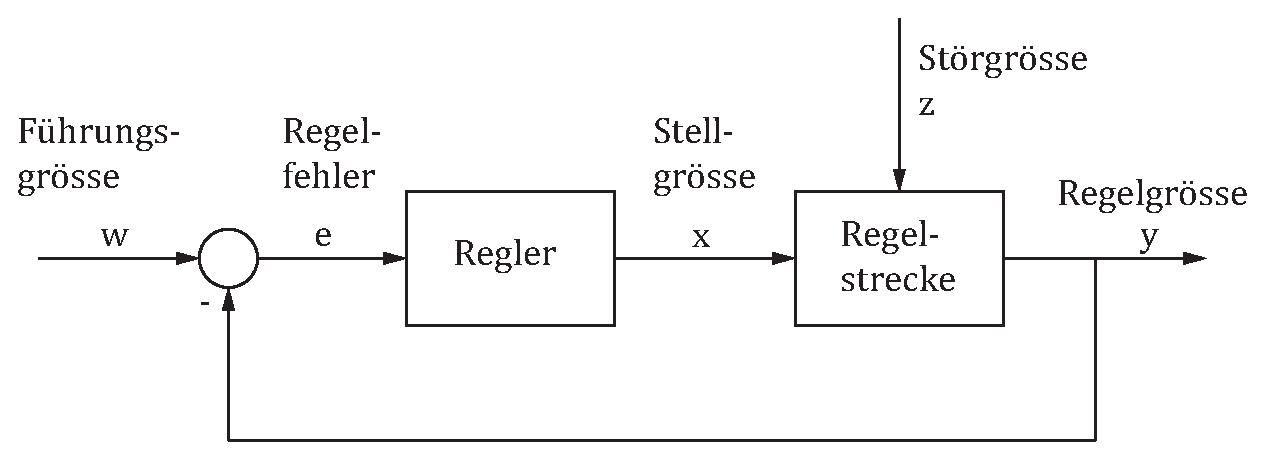
\includegraphics[width = \linewidth]{images/regelkreis.eps}
\\\\
Merkmale:
\begin{itemize}
	\item Erfassen der Regelgrösse $y$
	\item Vergleich von Führungs- und Regelgrösse
	\item Angleichen der Regelgrösse an die Führungsgrösse in Wirkungskreis
\end{itemize}
~\\
Führungsübertragungsverhalten:
\[
	G(s) = \frac{G_R \cdot G_S}{1 + G_R \cdot G_S}
\]
~\\
Störübertragungsverhalten (Störung zwischen Regler und Strecke):
\[
	G_{z1}(s) =\frac{G_S}{1 + G_R \cdot G_S}
\]
~\\
Störübertragungsverhalten (Störung nach Strecke):
\[
	G_{z2}(s) = \frac{1}{1 + G_R \cdot G_S}
\]

\section{Systeme}
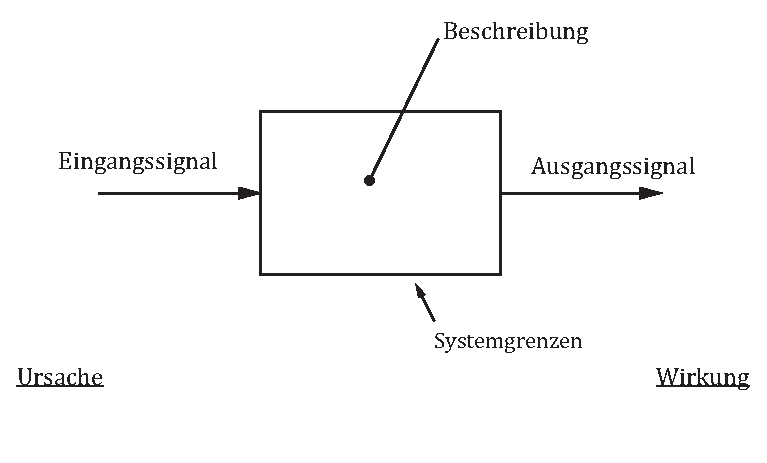
\includegraphics[width = \linewidth]{images/systeme.eps}
\\\\
Signale sind rückwirkungsfrei, also eingeprägte Grössen.
\\\\
\begin{center}
	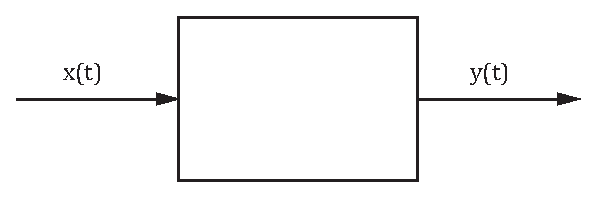
\includegraphics[scale = 0.5]{images/system_bsp.eps}
\end{center}
\newpage

\begin{tabular}{c|l|l}
 Nr. & Bsp & Klassifikation \\ 
\hline 1 & $y(t) = \cos t \cdot x(t)$ & statisch \\ 
	   2 & $\difrac{y(t)}{t} = - \cos (y(t)) + x(t)$ & \textbf{dynamisch} \\ 
\hline 3 & $\difrac{y(t)}{t} = -y(t) + x(t)$ & \textbf{zeitkontinierlich} \\ 
	   4 & $y((k+1)\tau)=-y(k\cdot \tau) + x(k \cdot \tau)$ & zeitdiskret \\ 
\hline 5 & $y(t) = \cos (x (t-\tau))$ & \textbf{kausal} \\ 
 	   6 & $y(t) = \cos(x(t+\tau))$ & nicht kausal \\ 
\hline 7 & $\difrac{y(t)}{t} = -3y(t) + x(t)$ & \textbf{zeitinvariant} \\ 
	   8 & $\difrac{y(t)}{t} = -\cos t \cdot y(t) +x(t)$ & zeitvariant \\ 
\hline 9 & $\difrac{y(t)}{t} = -y(t) +x(t)$ & \textbf{linear} \\ 
	   10 & $\difrac{y(t)}{t} = -y^2(t) +x(t)$ & nicht linear \\ 
\hline 11 & $\difrac{y(t)}{t} = -y(t) +x(t)$ & \textbf{endlich-dimensional} \\ 
	   12 & $\pdifrac{y(t)}{t} = - \pdifrac{}{x}y(x,t)+x(t)$ & unendlich-dimensional \\ 
\hline 13 & $y(t) = t \cdot \cos^2 t \cdot x(t)$ & \textbf{single input/output} \\ 
	   14 & $\left[ \begin{matrix} y_1(t) \\ y_2(t) \end{matrix}\right] = \left[ \begin{matrix} -3 & \sin(t) \\ t & -1\end{matrix}\right] \cdot \left[ \begin{matrix} x_1(t)\\ x_2(t) \end{matrix}\right]$ & multiple input/output \\ 
\end{tabular} 
\\\\

\section{Linearisierung}
Approximation durch Gerade:
\[
	f(\bar{x}+\Delta x) \approx \left.(\bar{x})+\difrac{f}{x}\right|_{\bar{x}}\cdot \Delta x
\]

\subsection{Arbeitspunkt festlegen}

Im stationären Zustand gilt:
\[
	\difrac{^n}{t^n} = 0
\]
~\\
Für das Eingangssignal $u(t)$ und das Ausgangssignal $y(t)$:
\[
	h(t) = \bar{y} + \Delta y(t) \qquad ,\ u(t) = \bar{u} + \Delta u(t)
\]


\subsection{Linearisierung um Arbeitspunkt}
Es gilt:
\[
	D(y^{(n)}, y^{(n-1)}, \dots ,\dot{y} ,y, u^{(m)}, u^{(m-1)}, \dots , \dot{u} ,u)= 0
\]
~\\
$D$ kann am Punkt $\bar{y}, \bar{u}$ approximiert werden durch:
\begin{small}
\[
	\left.\pdifrac{D}{y^{(n)}}\right|_{\begin{scriptsize}\begin{matrix} \bar{y} \\ \bar{u} \end{matrix}\end{scriptsize}} \cdot \Delta y^{n} + \dots +
	\left.\pdifrac{D}{\dot{y}}\right|_{\begin{scriptsize}\begin{matrix} \bar{y} \\ \bar{u} \end{matrix}\end{scriptsize}} \cdot \Delta \dot{y} +
	\left.\pdifrac{D}{y}\right|_{\begin{scriptsize}\begin{matrix} \bar{y} \\ \bar{u} \end{matrix}\end{scriptsize}} \cdot \Delta y +
	\left.\pdifrac{D}{u^{(n)}}\right|_{\begin{scriptsize}\begin{matrix} \bar{y} \\ \bar{u} \end{matrix}\end{scriptsize}} \cdot \Delta u^{n} + \dots +
	\left.\pdifrac{D}{u}\right|_{\begin{scriptsize}\begin{matrix} \bar{y} \\ \bar{u} \end{matrix}\end{scriptsize}} \cdot \Delta u = 0
\]
\end{small}

\begin{center}
	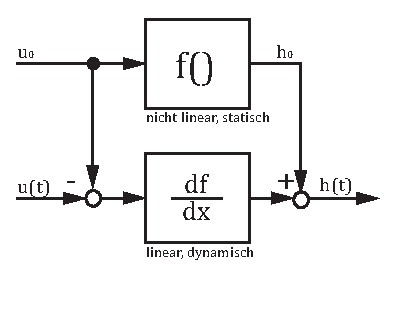
\includegraphics[scale = 0.8]{images/linearisierung.eps}
\end{center}

\section{Stabilität}
Grundlegendes Stabilitätskriterium für LZI-Glieder:\\
\begin{center}
\fbox{\parbox{.9\linewidth}{
	Ein LZI-Glied ist genau dann stabil, wenn die $n$ Nullstellen des Nennerpolynoms sämtliche negative Realteile haben. In der komplexen $s$-Ebene müssen die Nullstellen sämtlich links von der imaginären Achse liegen.
}}
\end{center}

\subsection{Hurwitz-Kriterium}
Das Polynom $N(s) = a_0 + a_1s + a_2s^2 + a_ns^n = 0$ ist nur dann stabil, 
wenn alle Koeffizienten $a_0, a_1, a_2, \ldots a_2$ \uline{ungleich null} sind und
ein \uline{positives Vorzeichen} haben. Zusätzlich müssen alle $n$ \uline{Linieardeterminanten positiv} sein (mit $n$ Zeilen und $n$ Spalten).  
\[
	D_n = \begin{vmatrix}
	a_1 & a_3 & a_5 & a_7 & \ldots \\ 
	a_0 & a_2 & a_4 & a_6 & \ldots \\ 
	0 & a_1 & a_3 & a_5 & \ldots \\ 
	0 & a_0 & a_2 & a_4 & \ldots \\ 
	0 & 0 & a_1 & a_3 & \ldots \\ 
	0 & 0 & a_0 & a_2 & \ldots \\
	\ldots
	\end{vmatrix} 
\]\\
Mit den jeweiligen Unterdeterminanten (für den fall $n=3$):\\
\[\begin{aligned}
	D_1 &= \begin{vmatrix}
		a_1 
		\end{vmatrix} = a_1 > 0\\
	D_2 &= \begin{vmatrix}
		a_1 & a_3 \\
		a_0 & a_2
	\end{vmatrix} = a_1a_2 - a_3a_0 > 0\\
	D_3 &= \begin{vmatrix}
		a_1 & a_3 & 0\\
		a_0 & a_2 & 0\\
		0	& a_1 & a_3
	\end{vmatrix} = a_3 D_2 > 0
\end{aligned}\]\\
Die letzte Determinante erfüllt jeweils zwangsmässig die Bedingung.

\subsection{Nyquist-Kriterium}
Das Stabilitätskriterium nach Nyquist beurteil die Stabilität eines Regelkreises aus dem Velrauf des \textbf{Frequenzgangs des offenen Regelkreises}.
Das Nyquist-Kriterium betrachtet die Ortskurve gegenüber dem Punkt $-1$ auf der reelen Achse. Dabei wird die Winkeländerung von $\omega = 0 \rightarrow \omega = \infty$ betrachtet. Dabei muss folgende Beziehung erfüllt sein, damit das Regelsystem stabil ist:
\[
	\Delta \varphi = i_k \cdot \frac{\pi}{2} + r_k \cdot \pi
\]\\
\begin{footnotesize}
	$r_k$: Anzahl Polstellen mit positivem Realteil\\
	$i_k$: Anzahl Polstellen auf der imaginären Achse
\end{footnotesize}

\begin{center}
	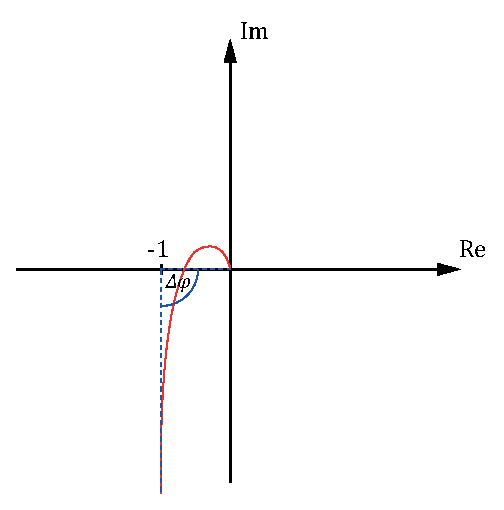
\includegraphics[scale=0.7]{images/nyquist.eps}
\end{center}

\section{Amplituden- und Phasenreserve}
Die Amplitudenreserve $A_R$ ist ein Mass für den Abstand der Ortskurve $G_O(\im\omega)$ vom Punkt $-1$ in Richtung der reelen Achse. Die Kreisfrequenz an der Stelle, an der $G_O(\im\omega)$ die reelle Achse schneidet, heisst Phasenschnittkreisfrequenz $\omega_\pi$.\\
Definition Amplitudenreserve:
\[
	A_R = \frac{1}{\left|G_O(\im\omega_\pi)\right|} \qquad \text{Stabilitätsbedingung: } A_R > 0.
\]\\\\
Die Phasenfrequenz $\varphi_R$ ist der Winkel zwischen der negativ-reellen Achse und dem Punkt, an dem die Ortskurve  $G_O(\im\omega)$ den Einheitskreis schneidet. Die Kreisfrequenz im Schnittpunkt heisst Durchtrittskreisfrequenz $\omega_D$.\\
Definition Phasenreserve:
\[
	\varphi_R = \angle{G_O(\im\omega_D)} + \pi \qquad \text{Stabilitätsbedingung: } \varphi > 0.
\]\\\\
Ablesen von der Ortskurve:
\begin{center}
	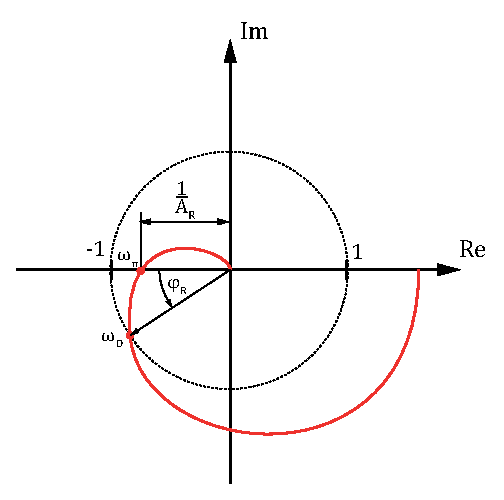
\includegraphics[scale=0.7]{images/ort_reserve.eps}
\end{center}
Ablesen vom Bodediagramm:
\begin{center}
	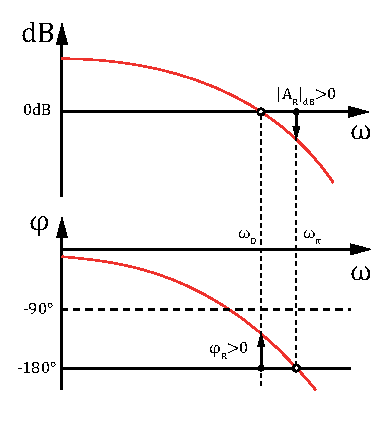
\includegraphics[scale=0.9]{images/bode_reserve.eps}
\end{center}

\subsection{Totzeitreserve}
Die Totzeitreserve $T_{tR}$ ist eine zusätzliche Totzeit, die in einem Regelkreis auftreten darf, ohne dass der Regelkreis instabil wird.\\
Definition Todzeitreserve:
\[
	T_{tR} = \frac{\varphi_R}{\omega_D}
\]
\section{Kompositionen von Grundelementen}

Betrachten der Verkettung:
\begin{center}
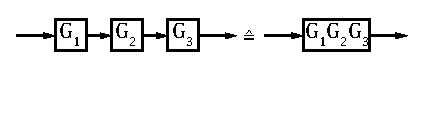
\includegraphics[scale = 1]{images/komp_grnd.eps}
\end{center}
Allgemeine Übertragungsfunktion:
\[
	G(s) = k \frac{s^n \cdot (1+sT_1)^n \ldots}{s^m \cdot (1+sT_2)^m(1+2dTs+s^2T^2)\ldots} \cdot \e^{-sT}
\]
\newpage

\begin{tabular}{>{\centering\arraybackslash}p{1.5cm}|>{\centering\arraybackslash}p{2.5cm}|>{\centering\arraybackslash}p{2cm}|>{\centering\arraybackslash}p{2.5cm}}
	   \rule[-2ex]{0pt}{5.5ex} Anteil  & Bode  & Ortskurve  & Sprungantwort  \\ 
\hline \rule[-2ex]{0pt}{5.5ex} $k$  & 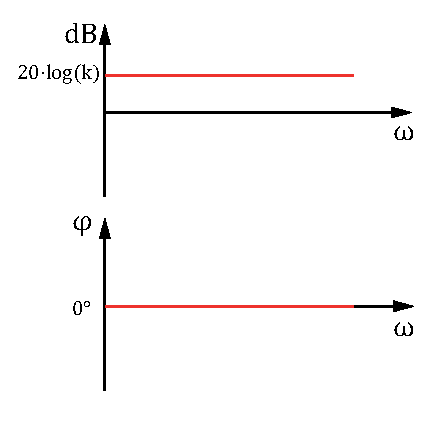
\includegraphics[scale = 0.3]{images/bode_k.eps} & 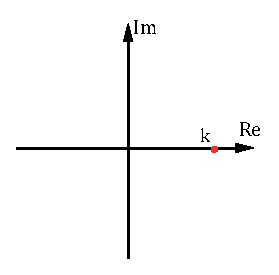
\includegraphics[scale = 0.4]{images/ort_k.eps} & 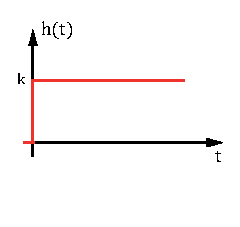
\includegraphics[scale = 0.5]{images/spr_k.eps} \\ 
\hline \rule[-2ex]{0pt}{5.5ex} $s^n$ & 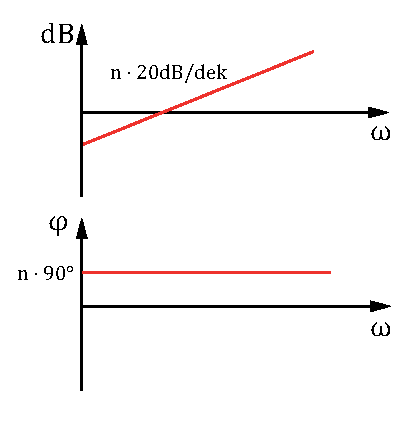
\includegraphics[scale = 0.3]{images/bode_sn.eps} & 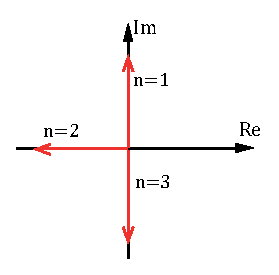
\includegraphics[scale = 0.4]{images/ort_sn.eps}  & 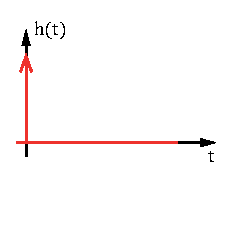
\includegraphics[scale = 0.5]{images/spr_sn.eps}  \\ 
\hline \rule[-2ex]{0pt}{5.5ex} $\frac{1}{s^m}$ & 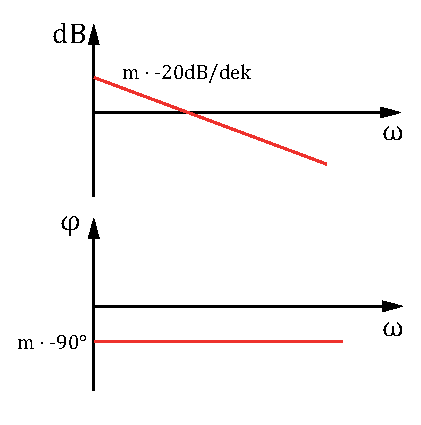
\includegraphics[scale = 0.3]{images/bode_sm.eps}  & 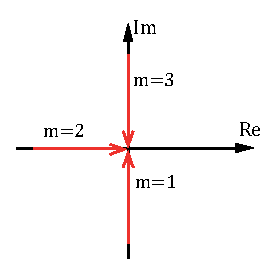
\includegraphics[scale = 0.4]{images/ort_sm.eps}  & 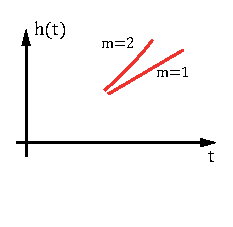
\includegraphics[scale = 0.5]{images/spr_sm.eps} \\ 
\hline \rule[-2ex]{0pt}{5.5ex} $(1+sT)^n$ & 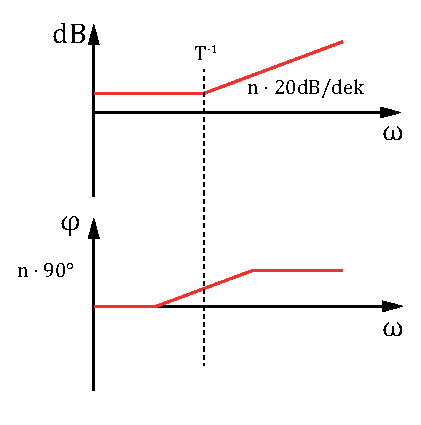
\includegraphics[scale = 0.3]{images/bode_1stn.eps} & 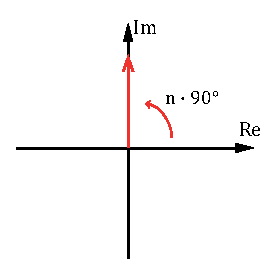
\includegraphics[scale = 0.4]{images/ort_1stn.eps}  & 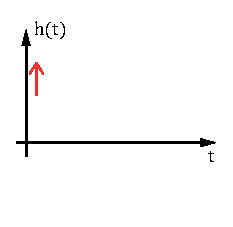
\includegraphics[scale = 0.5]{images/spr_1stn.eps} \\ 
\hline \rule[-2ex]{0pt}{5.5ex} $\frac{1}{(1+sT)^m}$ & 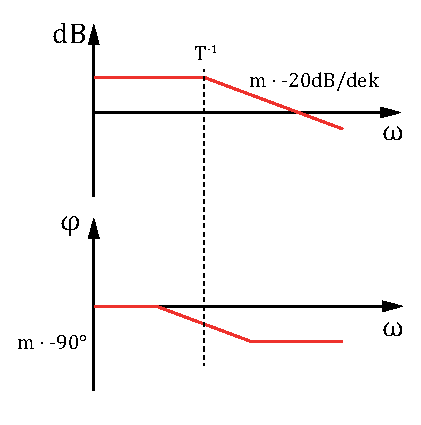
\includegraphics[scale = 0.3]{images/bode_1stm.eps} & 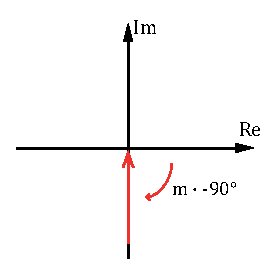
\includegraphics[scale = 0.4]{images/ort_1stm.eps} & 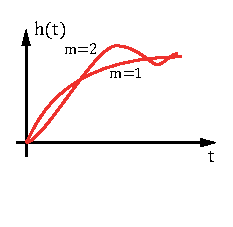
\includegraphics[scale = 0.5]{images/spr_1stm.eps} \\ 
\hline \rule[-2ex]{0pt}{5.5ex} $\e^{-sT}$ & 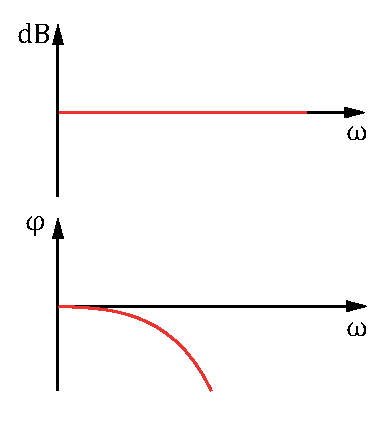
\includegraphics[scale = 0.3]{images/bode_est.eps} & 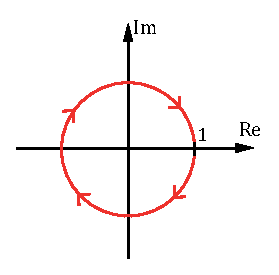
\includegraphics[scale = 0.4]{images/ort_est.eps} & 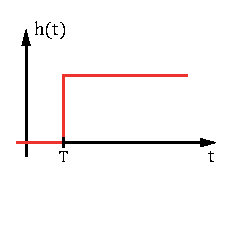
\includegraphics[scale = 0.5]{images/spr_est.eps} \\ 
\end{tabular} 

\section{Stationärer Fehler}
Der stationäre Fehler ist die Differenz zwischen Führungsgrüsse w(t) und Regelgrösse y(t) zum Zeitpunkt $t = \infty$:
\[
	e(\infty) = w(\infty) - y(\infty)
\]
~\\
Diese Grösse kann über den Laplace Endwertsatz berechnet werden:
\[
	 e(\infty) = \lim\limits_{s \rightarrow 0} s \cdot E(s) =  \lim\limits_{s \rightarrow 0} s \cdot \left(W(s) - Y(s)\right)
\]

\newpage

\section{Reglerelemente}
\subsection{Übersicht}
\begin{landscape}\centering
\begin{footnotesize}
\begin{longtable}{|c|c|c|c|c|c|}
\hline Name & $h(t)$ & $G(s)$ & Bode & Ortsk. & PN-Plan \\ 
\hline\endhead $P$ & 
	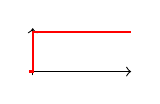
\begin{tikzpicture}[scale=.25]
		\draw[->] (-0.2,0) -- (5,0);
		\draw[->] (0,-0.2) -- (0,2.2);
		\draw[thick, red] (-0.2,0) -- (0,0) -- (0,2) -- (5,2);
	\end{tikzpicture} & $ K_P $ & 
	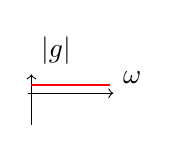
\begin{tikzpicture}[scale=.2]
        \draw[->] (-0.2,0) -- (5.2,0) node[above right] {$\omega$};
        \draw[->] (0,-2) -- (0,1.2) node[above right] {$|g|$};
        \draw[thick, red] (0,0.5) -- (5,0.5);
    \end{tikzpicture}
    \begin{tikzpicture}[scale=.2]
        \draw[->] (-0.2,0) -- (5.2,0) node[above right] {$\omega$};
        \draw[->] (0,-2) -- (0,1.2) node[above right] {$\varphi$};
        \draw[thick, red] (0,0) -- (5,0);
    \end{tikzpicture} & 
    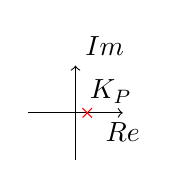
\begin{tikzpicture}[scale=0.3]
         \draw[->] (-2,0) -- (2,0) node[below] {$Re$};
         \draw[->] (0,-2) -- (0,2) node[above right] {$Im$};
         \node[above] at (1.5,0) {$K_P$};
         \draw[red] (.3,0.2) -- (.7,-0.2);
         \draw[red] (.3,-0.2) -- (.7,0.2);
     \end{tikzpicture} & $\nexists$ \\ 
\hline $PT_1$ & 
    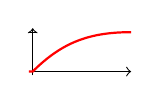
\begin{tikzpicture}[scale=.25]
        \draw[->] (-0.2,0) -- (5,0);
        \draw[->] (0,-0.2) -- (0,2.2);
        \draw[thick, red] (-0.2,0) -- (0,0) to[out=45, in=180] (5,2);
        \draw[-] (-0.2,2) -- (0.2,2);
    \end{tikzpicture} & $\frac{K_P}{1+sT_1}$ & 
    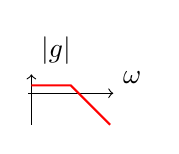
\begin{tikzpicture}[scale=.2]
        \draw[->] (-0.2,0) -- (5.2,0) node[above right] {$\omega$};
        \draw[->] (0,-2) -- (0,1.2) node[above right] {$|g|$};
        \draw[thick, red] (0,0.5) -- (2.5,0.5) -- (5,-2);
    \end{tikzpicture} 
    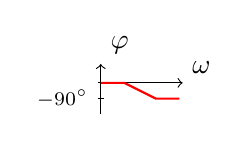
\begin{tikzpicture}[scale=.2]
        \draw[->] (-0.2,0) -- (5.2,0) node[above right] {$\omega$};
        \draw[->] (0,-2) -- (0,1.2) node[above right] {$\varphi$};
        \draw[thick, red] (0,0) -- (1.5,0) -- (3.5,-1) -- (5,-1);
        \draw[-] (-0.2,-1) node[left] {\scriptsize$-90^\circ$} -- (0.2,-1);
    \end{tikzpicture}& 
    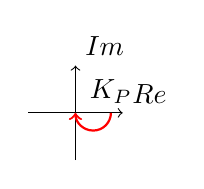
\begin{tikzpicture}[scale=.3]
        \draw[->] (-2,0) -- (2,0) node[above right] {$Re$};
        \draw[->] (0,-2) -- (0,2) node[above right] {$Im$};
        \draw[->, thick, red] (1.5,0) to[out=-90, in=0] (0.75,-0.75) to[out=180,in=-90] (0,0);
        \node[above] at (1.5,0){$K_P$};
    \end{tikzpicture} & 
    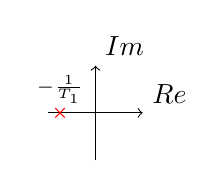
\begin{tikzpicture}[scale=.3]
        \draw[->] (-2,0) -- (2,0) node[above right] {$Re$};
        \draw[->] (0,-2) -- (0,2) node[above right] {$Im$};
        \draw[red] (-1.3,0.2) -- (-1.7,-0.2);
        \draw[red] (-1.3,-0.2) -- (-1.7,0.2);
        \node[above] at (-1.5,0) {\scriptsize$-\frac{1}{T_1}$};
    \end{tikzpicture} \\ 
\hline $PT_2$ & 
    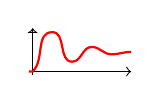
\begin{tikzpicture}[scale=.25]
        \draw[->] (-0.2,0) -- (5,0);
        \draw[->] (0,-0.2) -- (0,2.2);
        \draw[thick, red] (-0.2,0) -- (0,0) to[out=45, in=180] (1,2) to[out=0, in=180] (2,0.5) to[out=0, in=180] (3,1.25) to[out=0, in=180] (4,0.875) to[out=0, in=180] (5,1);
        \draw[-] (-0.2,2) -- (0.2,2);
    \end{tikzpicture} & $\frac{K_P \cdot {\omega_0}^2}{{\omega_0}^2 + 2d\omega_0\cdot s + s^2}$ & 
    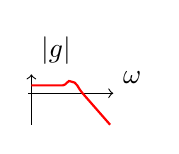
\begin{tikzpicture}[scale=.2]
        \draw[->] (-0.2,0) -- (5.2,0) node[above right] {$\omega$};
        \draw[->] (0,-2) -- (0,1.2) node[above right] {$|g|$};
        \draw[thick, red] (0,0.5) -- (2,0.5) to[out=0 in=180] (2.5,0.75) to[out=0, in=135] (3.25,0) -- (5,-2);
    \end{tikzpicture} 
    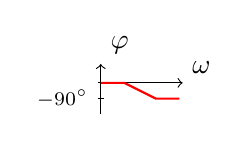
\begin{tikzpicture}[scale=.2]
        \draw[->] (-0.2,0) -- (5.2,0) node[above right] {$\omega$};
        \draw[->] (0,-2) -- (0,1.2) node[above right] {$\varphi$};
        \draw[thick, red] (0,0) -- (1.5,0) -- (3.5,-1) -- (5,-1);
        \draw[-] (-0.2,-1) node[left] {\scriptsize$-90^\circ$} -- (0.2,-1);
    \end{tikzpicture} & 
    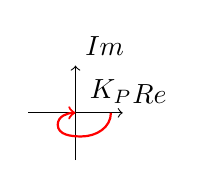
\begin{tikzpicture}[scale=.3]
        \draw[->] (-2,0) -- (2,0) node[above right] {$Re$};
        \draw[->] (0,-2) -- (0,2) node[above right] {$Im$};
        \draw[->, thick, red] (1.5,0) to[out=-90, in=0] (0.25,-1) to[out=180,in=-90] (-.75,-.5) to[out=90, in=180] (0,0);
        \node[above] at (1.5,0){$K_P$};
    \end{tikzpicture} & 
    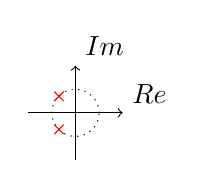
\begin{tikzpicture}[scale=.3]
        \draw[->] (-2,0) -- (2,0) node[above right] {$Re$};
        \draw[->] (0,-2) -- (0,2) node[above right] {$Im$};
        \draw[dotted] (0,0) circle (1);
        \draw[red] (-.5,.5) -- (-.9,.9);
        \draw[red] (-.5,.9) -- (-.9,.5);
        \draw[red] (-.5,-.5) -- (-.9,-.9);
        \draw[red] (-.5,-.9) -- (-.9,-.5);
    \end{tikzpicture} \\ 
\hline $PT_t$ & 
	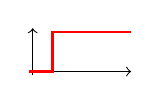
\begin{tikzpicture}[scale=.25]
		\draw[->] (-0.2,0) -- (5,0);
		\draw[->] (0,-0.2) -- (0,2.2);
		\draw[thick, red] (-0.2,0) -- (1,0) -- (1,2) -- (5,2);
	\end{tikzpicture} & $K_P \cdot \e^{-sT_t}$ & 
	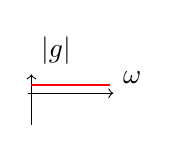
\begin{tikzpicture}[scale=.2]
	     \draw[->] (-0.2,0) -- (5.2,0) node[above right] {$\omega$};
	     \draw[->] (0,-2) -- (0,1.2) node[above right] {$|g|$};
	     \draw[thick, red] (0,0.5) -- (5,0.5);
	 \end{tikzpicture}
	 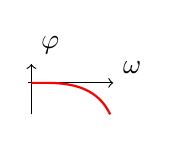
\begin{tikzpicture}[scale=.2]
	     \draw[->] (-0.2,0) -- (5.2,0) node[above right] {$\omega$};
	     \draw[->] (0,-2) -- (0,1.2) node[above right] {$\varphi$};
	     \draw[thick, red] (0,0) -- (1,0) to[out=0, in=115] (5,-2);
	 \end{tikzpicture} & 
	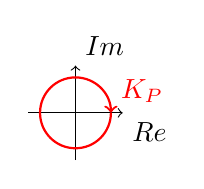
\begin{tikzpicture}[scale=.3]
        \draw[->] (-2,0) -- (2,0) node[below right] {$Re$};
        \draw[->] (0,-2) -- (0,2) node[above right] {$Im$};
        \draw[->, thick, red] (1.5,0) node[above right] {$K_P$} to[out=-90, in=0] (0,-1.5) to[out=180,in=-90] (-1.5,0) to[out=90, in=180] (0,1.5) to[out=0, in=90] (1.5,0);
    \end{tikzpicture} & $\nexists$ \\ 
\hline $D$ & 
    \begin{tikzpicture}[scale=.25]
        \draw[->] (-0.2,0) -- (5,0);
        \draw[->] (0,-0.2) -- (0,2.2);
        \draw[thick, red] (-0.2,0) -- (0,0);
        \draw[->, thick, red] (0,0) -- (0,1.5);
    \end{tikzpicture} & $K_D \cdot s$ & 
    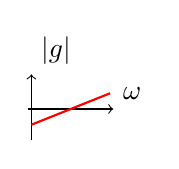
\begin{tikzpicture}[scale=.2]
        \draw[->] (-0.2,0) -- (5.2,0) node[above right] {$\omega$};
        \draw[->] (0,-2) -- (0,2.2) node[above right] {$|g|$};
        \draw[thick, red] (0,-1) -- (5,1);
    \end{tikzpicture}
    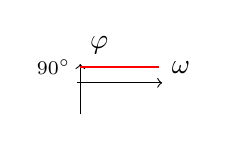
\begin{tikzpicture}[scale=.2]
        \draw[->] (-0.2,0) -- (5.2,0) node[above right] {$\omega$};
        \draw[->] (0,-2) -- (0,1.2) node[above right] {$\varphi$};
        \draw[thick, red] (0,1) -- (5,1);
        \node[left] at (0,1) {\scriptsize$90^\circ$};
    \end{tikzpicture} & 
    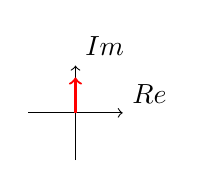
\begin{tikzpicture}[scale=.3]
        \draw[->] (-2,0) -- (2,0) node[above right] {$Re$};
        \draw[->] (0,-2) -- (0,2) node[above right] {$Im$};
        \draw[->, thick, red] (0,0) -- (0,1.5);
    \end{tikzpicture} & 
    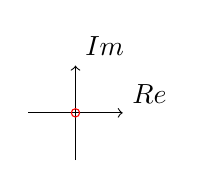
\begin{tikzpicture}[scale=.3]
        \draw[->] (-2,0) -- (2,0) node[above right] {$Re$};
        \draw[->] (0,-2) -- (0,2) node[above right] {$Im$};
        \draw[red] (0,0) circle (5pt);
    \end{tikzpicture} \\ 
\hline $DT_1$ & 
	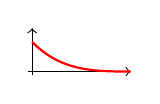
\begin{tikzpicture}[scale=.25]
	  \draw[->] (-0.2,0) -- (5,0);
	  \draw[->] (0,-0.2) -- (0,2.2);
	  \draw[thick, red] (0,1.5) to[out=-45, in=180] (5,0);
	\end{tikzpicture} & $\frac{K_D \cdot s}{1+ sT_1}$ & 
	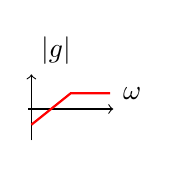
\begin{tikzpicture}[scale=.2]
		\draw[->] (-0.2,0) -- (5.2,0) node[above right] {$\omega$};
		\draw[->] (0,-2) -- (0,2.2) node[above right] {$|g|$};
		\draw[thick, red] (0,-1) -- (2.5,1) -- (5,1);
	\end{tikzpicture}
	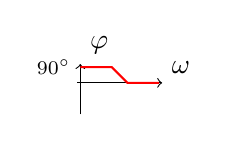
\begin{tikzpicture}[scale=.2]
		\draw[->] (-0.2,0) -- (5.2,0) node[above right] {$\omega$};
		\draw[->] (0,-2) -- (0,1.2) node[above right] {$\varphi$};
		\draw[thick, red] (0,1) -- (2,1) -- (3,0) -- (5,0);
		\node[left] at (0,1) {\scriptsize$90^\circ$};
	\end{tikzpicture} & 
	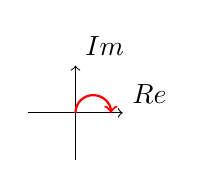
\begin{tikzpicture}[scale=.3]
	   \draw[->] (-2,0) -- (2,0) node[above right] {$Re$};
	   \draw[->] (0,-2) -- (0,2) node[above right] {$Im$};
	   \draw[->, thick, red] (0,0) to[out=90, in=180] (0.75,0.75) to[out=0, in=90] (1.5,0);
	\end{tikzpicture} & 
	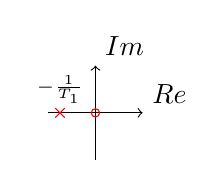
\begin{tikzpicture}[scale=.3]
		\draw[->] (-2,0) -- (2,0) node[above right] {$Re$};
		\draw[->] (0,-2) -- (0,2) node[above right] {$Im$};
		\draw[red] (0,0) circle (5pt);
		\draw[red] (-1.3,0.2) -- (-1.7,-0.2);
		\draw[red] (-1.3,-0.2) -- (-1.7,0.2);
		\node[above] at (-1.5,0) {\scriptsize$-\frac{1}{T_1}$};
	\end{tikzpicture} \\ 
\hline $PD$ & 
    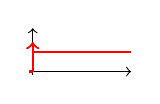
\begin{tikzpicture}[scale=.25]
        \draw[->] (-0.2,0) -- (5,0);
        \draw[->] (0,-0.2) -- (0,2.2);
        \draw[thick, red] (-0.2,0) -- (0,0);
        \draw[->, thick, red] (0,0) -- (0,1.5);
        \draw[thick, red] (0,1) -- (5,1);
    \end{tikzpicture} & $K_P \cdot (1+sT_V)$ & 
	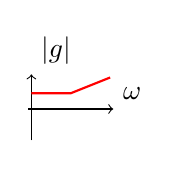
\begin{tikzpicture}[scale=.2]
		\draw[->] (-0.2,0) -- (5.2,0) node[above right] {$\omega$};
		\draw[->] (0,-2) -- (0,2.2) node[above right] {$|g|$};
		\draw[thick, red] (0,1) -- (2.5,1) -- (5,2);
	\end{tikzpicture}
	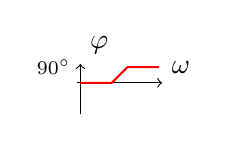
\begin{tikzpicture}[scale=.2]
		\draw[->] (-0.2,0) -- (5.2,0) node[above right] {$\omega$};
		\draw[->] (0,-2) -- (0,1.2) node[above right] {$\varphi$};
		\draw[thick, red] (0,0) -- (2,0) -- (3,1) -- (5,1);
		\node[left] at (0,1) {\scriptsize$90^\circ$};
	\end{tikzpicture} & 
	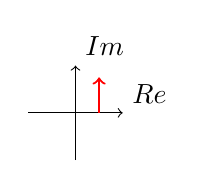
\begin{tikzpicture}[scale=.3]
		\draw[->] (-2,0) -- (2,0) node[above right] {$Re$};
		\draw[->] (0,-2) -- (0,2) node[above right] {$Im$};
		\draw[->, thick, red] (1,0) -- (1,1.5);
	\end{tikzpicture} & 
	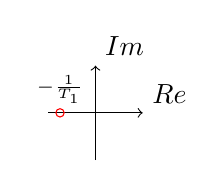
\begin{tikzpicture}[scale=.3]
		\draw[->] (-2,0) -- (2,0) node[above right] {$Re$};
		\draw[->] (0,-2) -- (0,2) node[above right] {$Im$};
		\draw[red] (-1.5,0) circle (5pt);
		\node[above] at (-1.5,0) {\scriptsize$-\frac{1}{T_1}$};
	\end{tikzpicture} \\ 
\hline $PDT_1$ & 
    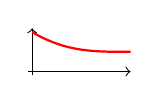
\begin{tikzpicture}[scale=.25]
        \draw[->] (-0.2,0) -- (5,0);
        \draw[->] (0,-0.2) -- (0,2.2);
        \draw[thick, red] (0,2) to[out=-30, in=180] (5,1);
    \end{tikzpicture} & $K_P \cdot \frac{1+T_V}{1+sT_1}$ , $T_V > T_1$ & 
   	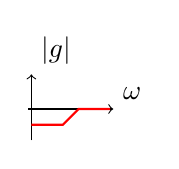
\begin{tikzpicture}[scale=.2]
   		\draw[->] (-0.2,0) -- (5.2,0) node[above right] {$\omega$};
   		\draw[->] (0,-2) -- (0,2.2) node[above right] {$|g|$};
   		\draw[thick, red] (0,-1) -- (2,-1) -- (3,0) -- (5,0);
   	\end{tikzpicture}
   	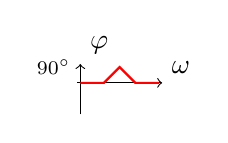
\begin{tikzpicture}[scale=.2]
   		\draw[->] (-0.2,0) -- (5.2,0) node[above right] {$\omega$};
   		\draw[->] (0,-2) -- (0,1.2) node[above right] {$\varphi$};
   		\draw[thick, red] (0,0) -- (1.5,0) -- (2.5,1) -- (3.5,0) -- (5,0);
   		\node[left] at (0,1) {\scriptsize$90^\circ$};
   	\end{tikzpicture} & 
	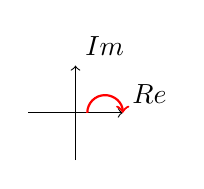
\begin{tikzpicture}[scale=.3]
		\draw[->] (-2,0) -- (2,0) node[above right] {$Re$};
		\draw[->] (0,-2) -- (0,2) node[above right] {$Im$};
		\draw[->, thick, red] (.5,0) to[out=90, in=180] (1.25,.75) to[out=0, in=90] (2,0);
	\end{tikzpicture} & 
	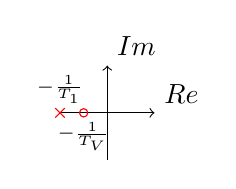
\begin{tikzpicture}[scale=.3]
		\draw[->] (-2,0) -- (2,0) node[above right] {$Re$};
		\draw[->] (0,-2) -- (0,2) node[above right] {$Im$};
		\draw[red] (-1,0) circle (5pt);
		\node[below] at (-1,0) {\scriptsize$-\frac{1}{T_V}$};
		\draw[red] (-2.2,0.2) -- (-1.8,-0.2);
		\draw[red] (-2.2,-0.2) -- (-1.8,0.2);
		\node[above] at (-2,0) {\scriptsize$-\frac{1}{T_1}$};
	\end{tikzpicture} \\ 
\hline $PPT_1$ & 
    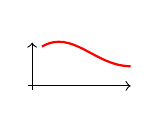
\begin{tikzpicture}[scale=.25]
        \draw[->] (-0.2,0) -- (5,0);
        \draw[->] (0,-0.2) -- (0,2.2);
        \draw[thick, red] (.5,2) to[out=30, in=180] (5,1);
    \end{tikzpicture} & $K_P \cdot \frac{1+T_V}{1+sT_1}$ , $T_V < T_1$ & 
   	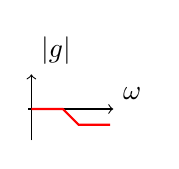
\begin{tikzpicture}[scale=.2]
   		\draw[->] (-0.2,0) -- (5.2,0) node[above right] {$\omega$};
   		\draw[->] (0,-2) -- (0,2.2) node[above right] {$|g|$};
   		\draw[thick, red] (0,0) -- (2,0) -- (3,-1) -- (5,-1);
   	\end{tikzpicture}
   	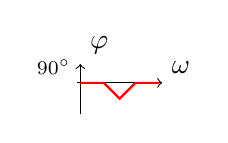
\begin{tikzpicture}[scale=.2]
   		\draw[->] (-0.2,0) -- (5.2,0) node[above right] {$\omega$};
   		\draw[->] (0,-2) -- (0,1.2) node[above right] {$\varphi$};
   		\draw[thick, red] (0,0) -- (1.5,0) -- (2.5,-1) -- (3.5,0) -- (5,0);
   		\node[left] at (0,1) {\scriptsize$90^\circ$};
   	\end{tikzpicture} & 
	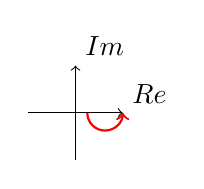
\begin{tikzpicture}[scale=.3]
		\draw[->] (-2,0) -- (2,0) node[above right] {$Re$};
		\draw[->] (0,-2) -- (0,2) node[above right] {$Im$};
		\draw[->, thick, red] (.5,0) to[out=-90, in=180] (1.25,-.75) to[out=0, in=-90] (2,0);
	\end{tikzpicture} & 
	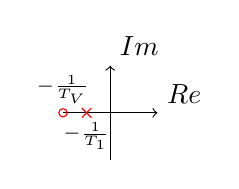
\begin{tikzpicture}[scale=.3]
		\draw[->] (-2,0) -- (2,0) node[above right] {$Re$};
		\draw[->] (0,-2) -- (0,2) node[above right] {$Im$};
		\draw[red] (-2,0) circle (5pt);
		\node[above] at (-2,0) {\scriptsize$-\frac{1}{T_V}$};
		\draw[red] (-1.2,0.2) -- (-.8,-0.2);
		\draw[red] (-1.2,-0.2) -- (-.8,0.2);
		\node[below] at (-1,0) {\scriptsize$-\frac{1}{T_1}$};
	\end{tikzpicture} \\ 
\hline $I$ & 
	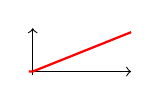
\begin{tikzpicture}[scale=.25]
        \draw[->] (-0.2,0) -- (5,0);
        \draw[->] (0,-0.2) -- (0,2.2);
        \draw[thick, red] (-0.2,0) -- (0,0) -- (5,2);
    \end{tikzpicture} & $K_I \cdot \frac{1}{s}$ & 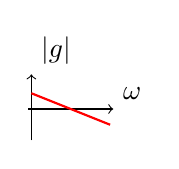
\begin{tikzpicture}[scale=.2]
		\draw[->] (-0.2,0) -- (5.2,0) node[above right] {$\omega$};
		\draw[->] (0,-2) -- (0,2.2) node[above right] {$|g|$};
		\draw[thick, red] (0,1) -- (5,-1);
	\end{tikzpicture}
	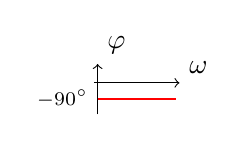
\begin{tikzpicture}[scale=.2]
	    \draw[->] (-0.2,0) -- (5.2,0) node[above right] {$\omega$};
	    \draw[->] (0,-2) -- (0,1.2) node[above right] {$\varphi$};
	    \draw[thick, red] (0,-1) -- (5,-1);
	    \node[left] at (0,-1) {\scriptsize$-90^\circ$};
	\end{tikzpicture} & 
	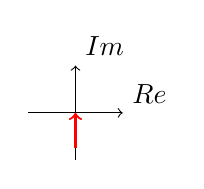
\begin{tikzpicture}[scale=.3]
        \draw[->] (-2,0) -- (2,0) node[above right] {$Re$};
        \draw[->] (0,-2) -- (0,2) node[above right] {$Im$};
        \draw[->, thick, red] (0,-1.5) -- (0,0);
    \end{tikzpicture} & 
    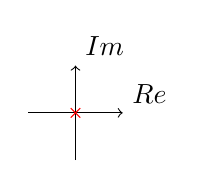
\begin{tikzpicture}[scale=.3]
		\draw[->] (-2,0) -- (2,0) node[above right] {$Re$};
		\draw[->] (0,-2) -- (0,2) node[above right] {$Im$};
		\draw[red] (.2,0.2) -- (-.2,-0.2);
		\draw[red] (.2,-0.2) -- (-.2,0.2);
	\end{tikzpicture} \\ 
\hline $IT_1$ & 
	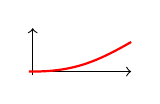
\begin{tikzpicture}[scale=.25]
        \draw[->] (-0.2,0) -- (5,0);
        \draw[->] (0,-0.2) -- (0,2.2);
        \draw[thick, red] (-0.2,0) -- (0,0) to[out=0, in=-150] (5,1.5);
    \end{tikzpicture} & $\frac{K_I}{s \cdot (1+sT_1)}$ & 
	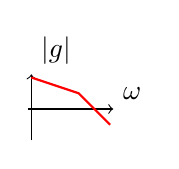
\begin{tikzpicture}[scale=.2]
		\draw[->] (-0.2,0) -- (5.2,0) node[above right] {$\omega$};
		\draw[->] (0,-2) -- (0,2.2) node[above right] {$|g|$};
		\draw[thick, red] (0,2) -- (3,1) -- (5,-1);
	\end{tikzpicture}
	\begin{tikzpicture}[scale=.2]
	    \draw[->] (-0.2,0) -- (5.2,0) node[above right] {$\omega$};
	    \draw[->] (0,-2) -- (0,1.2) node[above right] {$\varphi$};
	    \draw[thick, red] (0,-1) -- (2.5,-1) -- (3.5,-2) -- (5,-2);
	    \node[left] at (0,-1) {\scriptsize$-90^\circ$};
	\end{tikzpicture} & 
	\begin{tikzpicture}[scale=.3]
        \draw[->] (-2,0) -- (2,0) node[above right] {$Re$};
        \draw[->] (0,-2) -- (0,2) node[above right] {$Im$};
        \draw[->, thick, red] (-1,-2) to[out=90, in=180] (0,0);
    \end{tikzpicture} & 
    \begin{tikzpicture}[scale=.3]
		\draw[->] (-2,0) -- (2,0) node[above right] {$Re$};
		\draw[->] (0,-2) -- (0,2) node[above right] {$Im$};
		\draw[red] (.2,0.2) -- (-.2,-0.2);
		\draw[red] (.2,-0.2) -- (-.2,0.2);
		\draw[red] (-1.3,0.2) -- (-1.7,-0.2);
		\draw[red] (-1.3,-0.2) -- (-1.7,0.2);
		\node[above] at (-1.5,0) {\scriptsize$-\frac{1}{T_1}$};
	\end{tikzpicture} \\ 
\hline $PI$ & 
	\begin{tikzpicture}[scale=.25]
        \draw[->] (-0.2,0) -- (5,0);
        \draw[->] (0,-0.2) -- (0,2.2);
        \draw[thick, red] (-0.2,0) -- (0,0) -- (0,1) -- (5,2);
    \end{tikzpicture} & $K_P \cdot \left( 1 + \frac{1}{sT_N} \right)$ & 
	\begin{tikzpicture}[scale=.2]
		\draw[->] (-0.2,0) -- (5.2,0) node[above right] {$\omega$};
		\draw[->] (0,-2) -- (0,2.2) node[above right] {$|g|$};
		\draw[thick, red] (0,2) -- (2.5,1) -- (5,1);
	\end{tikzpicture}
	\begin{tikzpicture}[scale=.2]
	    \draw[->] (-0.2,0) -- (5.2,0) node[above right] {$\omega$};
	    \draw[->] (0,-2) -- (0,1.2) node[above right] {$\varphi$};
	    \draw[thick, red] (0,-1) -- (2,-1) -- (3,0) -- (5,0);
	    \node[left] at (0,-1) {\scriptsize$-90^\circ$};
	\end{tikzpicture} & 
	\begin{tikzpicture}[scale=.3]
        \draw[->] (-2,0) -- (2,0) node[above right] {$Re$};
        \draw[->] (0,-2) -- (0,2) node[above right] {$Im$};
        \draw[->, thick, red] (1,-2) -- (1,0);
    \end{tikzpicture} & 
	\begin{tikzpicture}[scale=.3]
		\draw[->] (-2,0) -- (2,0) node[above right] {$Re$};
		\draw[->] (0,-2) -- (0,2) node[above right] {$Im$};
		\draw[red] (.2,0.2) -- (-.2,-0.2);
		\draw[red] (.2,-0.2) -- (-.2,0.2);
		\draw[red] (-1.5,0) circle (5pt);
		\node[above] at (-1.5,0) {\scriptsize$-\frac{1}{T_1}$};
	\end{tikzpicture} \\ 
\hline $PID$ & 
	\begin{tikzpicture}[scale=.25]
        \draw[->] (-0.2,0) -- (5,0);
        \draw[->] (0,-0.2) -- (0,2.2);
        \draw[thick, red] (0,2) -- (0,1) -- (5,2);
    \end{tikzpicture} & $K_P \cdot \left( 1 + \frac{1}{sT_N} +sT_V \right)$ & 
	\begin{tikzpicture}[scale=.2]
		\draw[->] (-0.2,0) -- (5.2,0) node[above right] {$\omega$};
		\draw[->] (0,-2) -- (0,2.2) node[above right] {$|g|$};
		\draw[thick, red] (0,2) -- (2,1) -- (3,1) -- (5,2);
	\end{tikzpicture}
	\begin{tikzpicture}[scale=.2]
	    \draw[->] (-0.2,0) -- (5.2,0) node[above right] {$\omega$};
	    \draw[->] (0,-2) -- (0,1.2) node[above right] {$\varphi$};
	    \draw[thick, red] (0,-1) -- (1.5,-1) -- (3.5,1) -- (5,1);
	    \node[left] at (0,-1) {\scriptsize$-90^\circ$};
	\end{tikzpicture} & 
	\begin{tikzpicture}[scale=.3]
		\draw[->] (-2,0) -- (2,0) node[above right] {$Re$};
		\draw[->] (0,-2) -- (0,2) node[above right] {$Im$};
		\draw[->, thick, red] (1,-2) -- (1,2);
	\end{tikzpicture} & 
	\begin{tikzpicture}[scale=.3]
		\draw[->] (-2,0) -- (2,0) node[above right] {$Re$};
		\draw[->] (0,-2) -- (0,2) node[above right] {$Im$};
		\draw[red] (.2,0.2) -- (-.2,-0.2);
		\draw[red] (.2,-0.2) -- (-.2,0.2);
		\draw[red] (-1.5,0) circle (5pt);
		\draw[red] (-.75,0) circle (5pt);
	\end{tikzpicture} \\ 
\hline $PIDT_1$ & 
	\begin{tikzpicture}[scale=.25]
        \draw[->] (-0.2,0) -- (5,0);
        \draw[->] (0,-0.2) -- (0,2.2);
        \draw[thick, red] (0,2) to[out=-60, in=150] (0.75,1) to[out=-30, in=190] (2.5,1)-- (5,1.5);
    \end{tikzpicture} & $K_P \cdot \left( 1 + \frac{1}{sT_N} + \frac{sT_V}{1+sT_1} \right)$ & 
	\begin{tikzpicture}[scale=.2]
		\draw[->] (-0.2,0) -- (5.2,0) node[above right] {$\omega$};
		\draw[->] (0,-2) -- (0,2.2) node[above right] {$|g|$};
		\draw[thick, red] (0,2) -- (1,1) -- (2,1) -- (3,1.5) -- (5,1.5);
	\end{tikzpicture}
	\begin{tikzpicture}[scale=.2]
	    \draw[->] (-0.2,0) -- (5.2,0) node[above right] {$\omega$};
	    \draw[->] (0,-2) -- (0,1.2) node[above right] {$\varphi$};
	    \draw[thick, red] (0,-1) -- (.5,-1) -- (2.5,1) -- (3.5,0) -- (5,0);
	    \node[left] at (0,-1) {\scriptsize$-90^\circ$};
	    \node[left] at (0,1) {\scriptsize$90^\circ$};
	\end{tikzpicture} & 
	\begin{tikzpicture}[scale=.3]
		\draw[->] (-2,0) -- (2,0) node[above right] {$Re$};
		\draw[->] (0,-2) -- (0,2) node[above right] {$Im$};
		\draw[->, thick, red] (.5,-2) -- (.5,0) to[out=90, in=180] (1.25,0.75) to[out=0, in=90] (2,0);
	\end{tikzpicture} & 
	\begin{tikzpicture}[scale=.3]
		\draw[->] (-2,0) -- (2,0) node[above right] {$Re$};
		\draw[->] (0,-2) -- (0,2) node[above right] {$Im$};
		\draw[red] (.2,0.2) -- (-.2,-0.2);
		\draw[red] (.2,-0.2) -- (-.2,0.2);
		\draw[red] (-1.5,0) circle (5pt);
		\draw[red] (-.75,0) circle (5pt);
		\draw[red] (-2.2,0.2) -- (-1.8,-0.2);
		\draw[red] (-2.2,-0.2) -- (-1.8,0.2);
	\end{tikzpicture} \\ 
\hline 
\end{longtable} 
\end{footnotesize}
\end{landscape}
\clearpage

\subsection{$P$-Glied}
\begin{tabular}{ll}
\rule[-2ex]{0pt}{5.5ex} DGL: & $y(t) = K_P \cdot w(t)$ \\ 
\rule[-2ex]{0pt}{5.5ex} Übertragungsfunktion: & $G(s) = K_P$ \\ 
\rule[-2ex]{0pt}{5.5ex} Sprungantwort: & $h(t) = K_P$ \\ 
\end{tabular} 
~\\\\
\begin{tikzpicture}[scale=1]
	\draw[->] (-0.2,0) -- (5,0);
	\draw[->] (0,-0.2) -- (0,2.2);
	\draw[thick, red] (-0.2,0) -- (0,0) -- (0,1.8) -- (5,1.8);
	\node[left] at (0,1.8) {\small$K_P$};
\end{tikzpicture}
~\\\\
Bodediagramm:\\
\begin{tikzpicture}[scale=1]
    \draw[->] (-0.2,0) -- (5.2,0) node[above right] {\small$\omega$};
    \draw[->] (0,-1) -- (0,1.2) node[above left] {\small$\lg|G(\im\omega)|$};
    \draw[->] (4.9,-1) -- (4.9,1.2) node[above right] {\small$\varphi(\omega)$};
    \draw[thick, red] (0,0.5) -- (4.9,0.5);
    \node[above,red] at (2.5,0.5) {$\lg{K_P}$};
    \draw[thick, blue] (0,0) -- (4.9,0);
    \node[below,blue] at(2.5,0) {$\varphi$};
\end{tikzpicture}
~\\\\
\begin{tabular}{ll}
Ortskurve: & PN-Plan: \\ 
\begin{tikzpicture}[scale=.75]
     \draw[->] (-2,0) -- (2,0) node[below] {\small$Re$};
     \draw[->] (0,-2) -- (0,2) node[above right] {\small$Im$};
     \node[above right] at (.5,0) {\small$K_P$};
     \draw[red] (.3,0.2) -- (.7,-0.2);
     \draw[red] (.3,-0.2) -- (.7,0.2);
 \end{tikzpicture} & $\nexists$ \\ 
\end{tabular} 
\clearpage

\subsection{$PT_1$-Glied}
\begin{tabular}{ll}
\rule[-2ex]{0pt}{5.5ex} DGL: &  $T_1 \cdot \dot{y}(t) + y(t) = K_P \cdot u(t)$\\ 
\rule[-2ex]{0pt}{5.5ex} Übertragungsfunktion: & $G(s) = \frac{K_P}{1+sT_1}$ \\ 
\rule[-2ex]{0pt}{5.5ex} Sprungantwort: & $h(t) = K_P \cdot \left( 1 - \e^{-\frac{t}{T_1}} \right)$ \\ 
\end{tabular} 
~\\\\
\begin{tikzpicture}[scale=1]
    \draw[->] (-0.2,0) -- (5,0);
    \draw[->] (0,-0.2) -- (0,2.2);
    \draw[dotted] (0.1,2) -- (5,2);
    \draw[-] (0.1,2) -- (-0.1,2) node[left] {\small$K_P$};
    \draw[thick, red] (-0.2,0) -- (0,0) to[out=45, in=180] (5,2);
    \draw[dotted] (0,0) -- (2,2);
    \draw[dotted] (2,2) -- (2,1.4);
    \draw[<->] (2,0) -- (2,1.4);
    \draw[-] (2,.1) -- (2,-.1) node[below] {\small$T_1$};
    \node[right] at (2,.7) {\scriptsize$0.63\cdot K_P$};
\end{tikzpicture}
~\\\\
Bodediagramm:\\
\begin{tikzpicture}[scale=1]
    \draw[->] (-0.2,0) -- (5.2,0) node[above right] {\small$\omega$};
    \draw[->] (0,-1.5) -- (0,1.2) node[above left] {\small$\lg|G(\im\omega)|$};
    \draw[->] (4.9,-1.5) -- (4.9,1.2) node[above right] {\small$\varphi(\omega)$};
    \draw[thick, red] (0,1.1) to[out=0, in=135] (3.5,0.25) -- (4.9,-1.15);
    \draw[dotted] (0,1.1) -- (2.65,1.1) -- (4.9,-1.15);
    \draw[->] (1,0) -- (1,1.1);
    \node[left] at (1,0.5) {\scriptsize$\lg K_P$};
    \node[above right] at (3.5,.25) {\scriptsize$-20\frac{dB}{Dek}$};
    \draw[thick, blue] (0,0) to[out=0, in=135] (2.65,-.75) to[out=-45, in=180] (4.9,-1.5);
    \draw[dotted] (1.65,0) -- (3.65,-1.5) -- (4.9,-1.5);
    \draw[dotted] (2.65,1.1) node[above] {\scriptsize$\frac{1}{T_1}$} -- (2.65,-.75) -- (4.9,-.75);
    \draw[-] (4.9,-.75) -- (5,-.75) node[right] {\small$-45^\circ$};
    \draw[-] (4.9,-1.5) -- (5,-1.5) node[right] {\small$-90^\circ$};
    \draw[-] (1.65,.1) -- (1.65,0) node[below] {\scriptsize$0.1$};
    \draw[-] (2.65,.1) -- (2.65,0) node[below] {\scriptsize$1$};
    \draw[-] (3.65,.1) -- (3.65,0) node[below] {\scriptsize$10$};
\end{tikzpicture}
~\\\\
\begin{tabular}{ll}
Ortskurve: & PN-Plan: \\ 
\begin{tikzpicture}[scale=.75]
	\draw[->] (-2,0) -- (2,0) node[below] {\small$Re$};
	\draw[->] (0,-2) -- (0,2) node[above right] {\small$Im$};
	\draw[->, red] (1.5,0) to[out=-90, in=0] (.75,-.75);
	\draw[->, red] (.75,-.75) to[out=180, in=-90] (0,0);
	\draw[-] (.75,.1) node[above] {\scriptsize$K_P/2$} -- (.75,-.1);
	\draw[-] (-.1,-.75) node[left] {\scriptsize$K_P/2$} -- (.1,-.75);
	\draw[dotted] (.1,-.75) -- (.75,-.75) -- (.75,-.1);
\end{tikzpicture} & 
\begin{tikzpicture}[scale=.75]
	\draw[->] (-2,0) -- (2,0) node[below] {\small$Re$};
	\draw[->] (0,-2) -- (0,2) node[above right] {\small$Im$};
	\draw[-, red] (-.9,.1) -- (-1.1,-.1);
	\draw[-, red] (-.9,-.1) -- (-1.1,.1);
	\node[above] at (-1,0) {\small$-\frac{1}{T_1}$};
\end{tikzpicture} \\ 
\end{tabular} 
\clearpage

\subsection{$PT_2$-Glied}
\begin{tabular}{ll}
\rule[-2ex]{0pt}{5.5ex} DGL: & $\ddot{y}(t) + 2d\omega\cdot \dot{y}(t)+y=K_P \cdot u(t)$ \\ 
\rule[-2ex]{0pt}{5.5ex} Übertragungsfunktion: & $G(s) = \frac{K_P \cdot {\omega_0}^2}{{\omega_0}^2 + 2d\omega_0\cdot s + s^2}$ \\  
\end{tabular} 

\subsubsection{$D>1$ Kriechfall}
Sprungantwort: \qquad $h(t) = K_P \cdot \left( 1- \frac{T_1}{T_1-T_2} \cdot \e^{-\frac{t}{T_1}} + \frac{T_2}{T_1-T_2} \cdot \e^{-\frac{t}{T_2}} \right)$
~\\\\
\begin{tikzpicture}[scale=1]
    \draw[->] (-0.2,0) -- (5,0);
    \draw[->] (0,-0.2) -- (0,2.2);
    \draw[dotted] (0.1,2) -- (5,2);
    \draw[-] (0.1,2) -- (-0.1,2) node[left] {\small$K_P$};
    \draw[thick, red] (-0.2,0) -- (0,0) to[out=0, in=185] (5,2);
\end{tikzpicture}
~\\\\
Bodediagramm:\\
\begin{tikzpicture}[scale=1]
    \draw[->] (-0.2,0) -- (5.2,0) node[above right] {\small$\omega$};
    \draw[->] (0,-1.5) -- (0,1.2) node[above left] {\small$\lg|G(\im\omega)|$};
    \draw[->] (4.9,-1.5) -- (4.9,1.2) node[above right] {\small$\varphi(\omega)$};
    \draw[thick, red] (0,1.1) -- (1,1.1) to[out=0, in=150] (2.5,.5) -- (3.25,0) to[out=-30, in=120] (3.75,-.5) -- (4.3,-1.5);
    \draw[dotted] (0,1.1) -- (1.65,1.1) node[above] {\scriptsize$\frac{1}{T_1}$} -- (3.7,-.3) node[right] {\scriptsize$\frac{1}{T_2}$} -- (4.3,-1.5);
    \draw[->] (1,0) -- (1,1.1);
    \node[left] at (1,0.5) {\scriptsize$\lg K_P$};
    \node[above right] at (2.5,.25) {\scriptsize$-20\frac{dB}{Dek}$};
    \node[right] at (4,-1) {\scriptsize$-40\frac{dB}{Dek}$};
    \draw[thick, blue] (0,0) to[out=0, in=180] (4.9,-1.5);
    \draw[dotted] (.65,0) -- (4,-1.5) -- (4.9,-1.5);
    \draw[-] (4.9,-.75) -- (5,-.75) node[right] {\small$-90^\circ$};
    \draw[-] (4.9,-1.5) -- (5,-1.5) node[right] {\small$-180^\circ$};
    \draw[-] (.65,.1) -- (.65,0) node[below] {\scriptsize$0.1$};
    \draw[-] (1.65,.1) -- (1.65,0) node[below] {\scriptsize$1$};
    \draw[-] (2.65,.1) -- (2.65,0) node[below] {\scriptsize$10$};
\end{tikzpicture}
~\\\\
\begin{tabular}{ll}
Ortskurve: & PN-Plan: \\ 
\begin{tikzpicture}[scale=.75]
	\draw[->] (-2,0) -- (2,0) node[below] {\small$Re$};
	\draw[->] (0,-2) -- (0,2) node[above right] {\small$Im$};
	\draw[->, red] (1,0) to[out=-90, in=-30] (0,-.75) to[out=150, in=180] (0,0);
	\node[above] at (1,0) {\small$K_P$};
	\draw[-] (-.1,-.75) node[below left] {\scriptsize$-\frac{K_P}{2d}$} -- (.1,-.75) node[below right] {\scriptsize$\omega = \omega_0$};
\end{tikzpicture} & 
\begin{tikzpicture}[scale=.75]
	\draw[->] (-2,0) -- (2,0) node[below] {\small$Re$};
	\draw[->] (0,-2) -- (0,2) node[above right] {\small$Im$};
	\draw[-, red] (-.4,.1) -- (-.6,-.1);
	\draw[-, red] (-.4,-.1) -- (-.6,.1);
	\node[above] at (-.5,0) {\small$-\frac{1}{T_1}$};
	\draw[-, red] (-1.4,.1) -- (-1.6,-.1);
	\draw[-, red] (-1.4,-.1) -- (-1.6,.1);
	\node[above] at (-1.5,0) {\small$-\frac{1}{T_2}$};
\end{tikzpicture} \\ 
\end{tabular} 
\clearpage

\subsubsection{$D=1$ aperiodischer Grenzfall}
Sprungantwort: \qquad $h(t) = K_P \cdot \left( 1- \cdot \e^{-\frac{t}{T_1}} - \frac{t}{T_1} \cdot \e^{-\frac{t}{T_1}} \right)$
~\\\\
\begin{tikzpicture}[scale=1]
    \draw[->] (-0.2,0) -- (5,0);
    \draw[->] (0,-0.2) -- (0,2.2);
    \draw[dotted] (0.1,2) -- (5,2);
    \draw[-] (0.1,2) -- (-0.1,2) node[left] {\small$K_P$};
    \draw[thick, red] (-0.2,0) -- (0,0) to[out=0, in=185] (3,2) -- (5,2);
\end{tikzpicture}
~\\\\
Bodediagramm:\\
\begin{tikzpicture}[scale=1]
    \draw[->] (-0.2,0) -- (5.2,0) node[above right] {\small$\omega$};
    \draw[->] (0,-1.5) -- (0,1.2) node[above left] {\small$\lg|G(\im\omega)|$};
    \draw[->] (4.9,-1.5) -- (4.9,1.2) node[above right] {\small$\varphi(\omega)$};
    \draw[thick, red] (0,1.1) to[out=0, in=135] (3.5,0.25) -- (4.9,-1.15);
    \draw[dotted] (0,1.1) -- (2.65,1.1) -- (4.9,-1.15);
    \draw[->] (1,0) -- (1,1.1);
    \node[left] at (1,0.5) {\scriptsize$\lg K_P$};
    \draw[<->] (2.65,1.1) node[below right] {\scriptsize$-6dB$} -- (2.65,.85);
    \node[above right] at (3.5,.25) {\scriptsize$-40\frac{dB}{Dek}$};
    \draw[thick, blue] (0,0) to[out=0, in=135] (2.65,-.75) to[out=-45, in=180] (4.9,-1.5);
    \draw[dotted] (1.65,0) -- (3.65,-1.5) -- (4.9,-1.5);
    \draw[dotted] (2.65,1.1) node[above] {\scriptsize$\frac{1}{T_1}$} -- (2.65,-.75) -- (4.9,-.75);
    \draw[-] (4.9,-.75) -- (5,-.75) node[right] {\small$-90^\circ$};
    \draw[-] (4.9,-1.5) -- (5,-1.5) node[right] {\small$-180^\circ$};
    \draw[-] (1.65,.1) -- (1.65,0) node[below] {\scriptsize$0.1\omega_0$};
    \draw[-] (2.65,.1) -- (2.65,0) node[below] {\scriptsize$\omega_0$};
    \draw[-] (3.65,.1) -- (3.65,0) node[below] {\scriptsize$10\omega_0$};
\end{tikzpicture}
~\\\\
\begin{tabular}{ll}
Ortskurve: & PN-Plan: \\ 
\begin{tikzpicture}[scale=.75]
	\draw[->] (-2,0) -- (2,0) node[below] {\small$Re$};
	\draw[->] (0,-2) -- (0,2) node[above right] {\small$Im$};
	\draw[->, red] (1,0) to[out=-90, in=-30] (0,-.75) to[out=150, in=180] (0,0);
	\node[above] at (1,0) {\small$K_P$};
	\draw[-] (-.1,-.75) node[below left] {\scriptsize$-\frac{K_P}{2}$} -- (.1,-.75) node[below right] {\scriptsize$\omega = \omega_0$};
\end{tikzpicture} & 
\begin{tikzpicture}[scale=.75]
	\draw[->] (-2,0) -- (2,0) node[below] {\small$Re$};
	\draw[->] (0,-2) -- (0,2) node[above right] {\small$Im$};
	\draw[-, red] (-1.05,.1) -- (-.85,-.1);
	\draw[-, red] (-1.05,-.1) -- (-.85,.1);
	\draw[-, red] (-1.15,.1) -- (-.95,-.1);
	\draw[-, red] (-1.15,-.1) -- (-.95,.1);
	\node[above] at (-1,0) {\small$-\frac{1}{T_1}$};
\end{tikzpicture} \\ 
\end{tabular} 
\clearpage


\subsubsection{$0<D<1$ stabiler Schwingfall}
Sprungantwort: \qquad $h(t) = K_P \cdot \left( 1- \frac{\e^{-d\omega_0t}}{\sqrt{1-d^2}} \cdot \sin\left(\omega_et + \arccos d \right) \right)$\\
Eigenkreisfrequenz: $\ \omega_e=\sqrt{1-d^2}\cdot \omega_0$\\
Peridoendauer: \qquad $T_P = \frac{2\pi}{\omega_e}$
~\\\\
\begin{tikzpicture}[scale=1]
    \draw[->] (-0.2,0) -- (5,0);
    \draw[->] (0,-0.2) -- (0,2.2);
    \draw[dotted] (0.1,1.5) -- (5,1.5);
    \draw[-] (0.1,1.5) -- (-0.1,1.5) node[left] {\small$K_P$};
    \draw[domain=0:5,variable=\t,thick,red] plot[samples=500] ({\t},{1.5 * (1-exp(-0.2*7.255*\t)/sqrt(1-0.2^2)*sin(deg(sqrt(1-0.2^2)*7.255*\t+1.37))});   
    \draw[dotted] (.7,1.5) -- (.7,2.2);
    \draw[dotted] (1.6,1.5) -- (1.6,2.2);
    \draw[<->] (.7,2) -- (1.6,2);
    \node[above] at (1.2,2) {\scriptsize$T_P$};
\end{tikzpicture}
~\\\\
Bodediagramm:\\
\begin{tikzpicture}[scale=1]
    \draw[->] (-0.2,0) -- (5.2,0) node[above right] {\small$\omega$};
    \draw[->] (0,-1.5) -- (0,1.2) node[above left] {\small$\lg|G(\im\omega)|$};
    \draw[->] (4.9,-1.5) -- (4.9,1.2) node[above right] {\small$\varphi(\omega)$};  
    \draw[scale=2,domain=0:1.85,variable=\x,thick,red] plot[samples=500] ({\x},{.25-log10(sqrt((1-(10^(\x)/21.13)^2)^2+(2*.2*10^(\x)/21.13)^2))});
    \draw[dotted] (0,.5) -- (2.65,.5) -- (3.7,-1.6);
    \draw[<->] (1,0) -- (1,.5);
    \node[left] at (1,.25) {\scriptsize$\lg K_P$};
    \node[above right] at (3.5,.25) {\scriptsize$-40\frac{dB}{Dek}$};
    \draw[thick, blue] (0,0) to[out=0, in=110] (2.65,-.75) to[out=-70, in=180] (4.9,-1.5);
    \draw[dotted] (1.65,0) -- (3.65,-1.5) -- (4.9,-1.5);
    \draw[dotted] (2.65,.5) -- (2.65,-.75) -- (4.9,-.75);
    \draw[-] (4.9,-.75) -- (5,-.75) node[right] {\small$-90^\circ$};
    \draw[-] (4.9,-1.5) -- (5,-1.5) node[right] {\small$-180^\circ$};
    \draw[-] (1.65,.1) -- (1.65,0) node[below] {\scriptsize$0.1 \omega_0$};
    \draw[-] (2.65,.1) -- (2.65,0) node[below] {\scriptsize$\omega_0$};
    \draw[-] (3.65,.1) -- (3.65,0) node[below] {\scriptsize$10 \omega_0$};
\end{tikzpicture}
~\\\\
\begin{tabular}{ll}
Ortskurve: & PN-Plan: \\ 
\begin{tikzpicture}[scale=.75]
	\draw[->] (-2,0) -- (2,0) node[below] {\small$Re$};
	\draw[->] (0,-2) -- (0,2) node[above right] {\small$Im$};
	\draw[->, red] (1,0) to[out=-90, in=-30] (0,-.75) to[out=150, in=180] (0,0);
	\node[above] at (1,0) {\small$K_P$};
	\draw[-] (-.1,-.75) node[below left] {\scriptsize$-\frac{K_P}{2d}$} -- (.1,-.75) node[below right] {\scriptsize$\omega = \omega_0$};
\end{tikzpicture} & 
\begin{tikzpicture}[scale=.75]
	\draw[->] (-2,0) -- (2,0) node[below] {\small$Re$};
	\draw[->] (0,-2) -- (0,2) node[above right] {\small$Im$};
	\draw[thick] (0,0) circle (1.5);
	\draw[thick, red] (-1.16,1.16) -- (-.96,.96);
	\draw[thick, red] (-1.16,.96) -- (-.96,1.16);
	\draw[thick, red] (-1.16,-1.16) -- (-.96,-.96);
	\draw[thick, red] (-1.16,-.96) -- (-.96,-1.16);
	\node[above left] at(0,1.5) {\scriptsize$w_0$};
	\node[above right] at(1.5,0) {\scriptsize$w_0$};
	\node[below left] at(0,-1.5) {\scriptsize$-w_0$};
	\node[above left] at(-1.5,0) {\scriptsize$-w_0$};
	\draw[dotted] (0,1.06) -- (-1.06,1.06) -- (-1.06,-1.06) -- (0,-1.06);
	\draw[-] (-.1,1.06) -- (.1,1.06) node[right] {\scriptsize$\omega_0\sqrt{1-d^2}$};
	\draw[-] (-.1,-1.06) -- (.1,-1.06) node[right] {\scriptsize$\omega_0\sqrt{1-d^2}$};
	\draw[-] (-1.06,.1) -- (-1.06,-.1) node[below] {\scriptsize$-\omega_0d$};
	\draw[-] (0,0) -- (-1.06,1.06);
	\draw[-] (-.5,0) to[out=90, in=235] (-.38,.38);
	\node at (-.26, .1) {\tiny$\alpha$};
	\node[above right] at (-.1,0) {\tiny$\cos\alpha = d$};
\end{tikzpicture} \\ 
\end{tabular} 
\clearpage

\subsubsection{$D=0$ grenzstabiler Schwingfall}
Sprungantwort: \qquad $h(t) = K_P \cdot \left( 1- \cos\omega_0t \right)$\\
Eigenkreisfrequenz: $\ \omega_e=\omega_0$\\
Peridoendauer: \qquad $T_P = \frac{2\pi}{\omega_0}$
~\\\\
\begin{tikzpicture}[scale=1]
    \draw[->] (-0.2,0) -- (5,0);
    \draw[->] (0,-0.2) -- (0,2.2);
    \draw[dotted] (0.1,1) -- (5,1);
    \draw[-] (0.1,1) -- (-0.1,1) node[left] {\small$K_P$};
    \draw[dotted] (0.1,2) -- (5,2);
    \draw[-] (0.1,2) -- (-0.1,2) node[left] {\small$2K_P$};
    \draw[domain=0:5,variable=\t,thick,red] plot[samples=500] ({\t},{1 * (1 - cos(deg(6.28*\t))});   
    \draw[dotted] (.5,2) -- (.5,2.5);
    \draw[dotted] (1.5,2) -- (1.5,2.5);
    \draw[<->] (.5,2.3) -- (1.5,2.3);
    \node[above] at (1.2,2.3) {\scriptsize$T_P$};
\end{tikzpicture}
~\\\\
Bodediagramm:\\
\begin{tikzpicture}[scale=1]
    \draw[->] (-0.2,0) -- (5.2,0) node[above right] {\small$\omega$};
    \draw[->] (0,-1.5) -- (0,1.2) node[above left] {\small$\lg|G(\im\omega)|$};
    \draw[->] (4.9,-1.5) -- (4.9,1.2) node[above right] {\small$\varphi(\omega)$};  
    \draw[scale=2,domain=0:1.2,variable=\x,thick,red] plot[samples=500] ({\x},{.25-log10(sqrt((1-(10^(\x)/21.13)^2)^2))});
    \draw[scale=2,domain=1.405:1.85,variable=\x,thick,red] plot[samples=500] ({\x},{.25-log10(sqrt((1-(10^(\x)/21.13)^2)^2))});
    \draw[dotted] (0,.5) -- (2.65,.5) -- (3.7,-1.6);
    \draw[<->] (1,0) -- (1,.5);
    \node[left] at (1,.25) {\scriptsize$\lg K_P$};
    \node[above right] at (3.5,.25) {\scriptsize$-40\frac{dB}{Dek}$};
    \draw[thick, blue] (0,0) -- (5,0);
    \draw[-] (4.9,-.75) -- (5,-.75) node[right] {\small$-90^\circ$};
    \draw[-] (4.9,-1.5) -- (5,-1.5) node[right] {\small$-180^\circ$};
    \draw[-] (1.65,.1) -- (1.65,0) node[below] {\scriptsize$0.1 \omega_0$};
    \draw[-] (2.65,.1) -- (2.65,0) node[below] {\scriptsize$\omega_0$};
    \draw[-] (3.65,.1) -- (3.65,0) node[below] {\scriptsize$10 \omega_0$};
\end{tikzpicture}
~\\\\
\begin{tabular}{ll}
Ortskurve: & PN-Plan: \\ 
\begin{tikzpicture}[scale=.75]
	\draw[->] (-2,0) -- (2,0) node[below] {\small$Re$};
	\draw[->] (0,-2) -- (0,2) node[above right] {\small$Im$};
	\draw[->, thick, red] (1,0) -- (0,0);
	\node[above] at (1,0) {\small$K_P$};
\end{tikzpicture} & 
\begin{tikzpicture}[scale=.75]
	\draw[->] (-2,0) -- (2,0) node[below] {\small$Re$};
	\draw[->] (0,-2) -- (0,2) node[above right] {\small$Im$};
	\draw[thick] (0,0) circle (1.5);
	\draw[thick, red] (-.1,1.4) -- (.1,1.6);
	\draw[thick, red] (-.1,1.6) -- (.1,1.4);
	\draw[thick, red] (-.1,-1.4) -- (.1,-1.6);
	\draw[thick, red] (-.1,-1.6) -- (.1,-1.4);
	\node[above left] at(0,1.5) {\scriptsize$w_0$};
	\node[above right] at(1.5,0) {\scriptsize$w_0$};
	\node[below left] at(0,-1.5) {\scriptsize$-w_0$};
	\node[above left] at(-1.5,0) {\scriptsize$-w_0$};
\end{tikzpicture} \\ 
\end{tabular} 
\clearpage

\subsection{$PT_t$-Glied}
\begin{tabular}{ll}
\rule[-2ex]{0pt}{5.5ex} DGL: & $y(t) = K_P \cdot u(t-T_t)$ \\ 
\rule[-2ex]{0pt}{5.5ex} Übertragungsfunktion: & $G(s) =K_P \cdot \e^{-sT_t}$ \\ 
\rule[-2ex]{0pt}{5.5ex} Sprungantwort: & $h(t) = K_P \cdot \sigma(t-T_t)$ \\
\end{tabular}
~\\\\
\begin{tikzpicture}[scale=1]
    \draw[->] (-0.2,0) -- (5,0);
    \draw[->] (0,-0.2) -- (0,2.2);
    \draw[dotted] (0.1,1.5) -- (5,1.5);
    \draw[-] (0.1,1.5) -- (-0.1,1.5) node[left] {\small$K_P$};
    \draw[thick,red] (-.2,0) -- (2,0) -- (2,1.5) -- (5,1.5);   
    \draw[dotted] (0,0) -- (0,-.5);
    \draw[dotted] (2,0) -- (2,-.5);
    \draw[<->] (0,-.25) -- (2,-.25);
    \node[below] at (1,-.25) {\scriptsize$T_t$};
\end{tikzpicture}
~\\\\
Bodediagramm:\\
\begin{tikzpicture}[scale=1]
    \draw[->] (-0.2,0) -- (5.2,0) node[above right] {\small$\omega$};
    \draw[->] (0,-1.5) -- (0,1.2) node[above left] {\small$\lg|G(\im\omega)|$};
    \draw[->] (4.9,-1.5) -- (4.9,1.2) node[above right] {\small$\varphi(\omega)$};  
	\draw[thick,red] (0,.8) -- (5,.8);
    \draw[<->] (1,0) -- (1,.8);
    \node[left] at (1,.4) {\scriptsize$\lg K_P$};
    \draw[thick, blue] (0,0) -- (1,0) to[out=0, in=115] (4,-1.5);
\end{tikzpicture}
~\\\\
\begin{tabular}{ll}
Ortskurve: & PN-Plan: \\ 
\begin{tikzpicture}[scale=.75]
	\draw[->] (-2,0) -- (2,0) node[below] {\small$Re$};
	\draw[->] (0,-2) -- (0,2) node[above right] {\small$Im$};
	\draw[->, thick, red] (1.5,0) to[out=-90, in=0] (0,-1.5) to[out=180,in=-90] (-1.5,0) to[out=90, in=180] (0,1.5) to[out=0, in=90] (1.5,0);
	\draw[-] (1.5,.1) -- (1.5,-.1);
	\node[above left] at (1.5,0) {\small$K_P$};
\end{tikzpicture} & $\nexists$\\ 
\end{tabular} 
\clearpage

 
\subsection{$D$-Glied}
\begin{tabular}{ll}
\rule[-2ex]{0pt}{5.5ex} DGL: & $y(t) = K_D \cdot \dot{u}(t)$ \\ 
\rule[-2ex]{0pt}{5.5ex} Übertragungsfunktion: & $G(s) = K_P \cdot s$ \\ 
\rule[-2ex]{0pt}{5.5ex} Sprungantwort: & $h(t) = K_P \cdot \delta(t)$ \\ 
\end{tabular} 
~\\\\
\begin{tikzpicture}[scale=1]
    \draw[->] (-0.2,0) -- (5,0);
    \draw[->] (0,-0.2) -- (0,2.2);
    \draw[thick,red] (-.2,0) -- (5,0);
    \draw[->,thick,red] (0,0) -- (0,2) node[left] {\scriptsize$K_P$};
\end{tikzpicture}
~\\\\
Bodediagramm:\\
\begin{tikzpicture}[scale=1]
    \draw[->] (-0.2,0) -- (5.2,0) node[above right] {\small$\omega$};
    \draw[->] (0,-1.5) -- (0,1.2) node[above left] {\small$\lg|G(\im\omega)|$};
    \draw[->] (4.9,-1.5) -- (4.9,1.2) node[above right] {\small$\varphi(\omega)$};  
	\draw[thick, red] (0,-1) -- (4.9,1);
	\draw[-] (2.45,.1) -- (2.45,-.1) node[below] {\scriptsize$\frac{1}{K_P}$};
	\node[below] at (4,.5) {\scriptsize$20\frac{dB}{Dek}$};
	\draw[thick, blue] (0,1) -- (4.9,1);
	\node[right] at (4.9,1) {\scriptsize$90^\circ$};
\end{tikzpicture}
~\\\\
\begin{tabular}{ll}
Ortskurve: & PN-Plan: \\ 
\begin{tikzpicture}[scale=.75]
	\draw[->] (-2,0) -- (2,0) node[below] {\small$Re$};
	\draw[->] (0,-2) -- (0,2) node[above right] {\small$Im$};
	\draw[->, thick, red] (0,0) -- (0,1.5);
\end{tikzpicture} & 
\begin{tikzpicture}[scale=.75]
    \draw[->] (-2,0) -- (2,0) node[above right] {$Re$};
    \draw[->] (0,-2) -- (0,2) node[above right] {$Im$};
    \draw[red] (0,0) circle (2.5pt);
\end{tikzpicture}\\ 
\end{tabular} 
\clearpage


\subsection{$DT_1$-Glied}
\begin{tabular}{ll}
\rule[-2ex]{0pt}{5.5ex} DGL: & $T_1 \cdot \dot{y}(t) + y(t) = K_D \cdot \dot{u}(t)$ \\ 
\rule[-2ex]{0pt}{5.5ex} Übertragungsfunktion: & $G(s) = \frac{K_D \cdot s}{1+ sT_1}$ \\ 
\rule[-2ex]{0pt}{5.5ex} Sprungantwort: & $h(t) = \frac{K_D}{T_1} \cdot \e^{-\frac{t}{T_1}}$ \\ 
\end{tabular} 
~\\\\
\begin{tikzpicture}[scale=1]
    \draw[->] (-0.2,0) -- (5,0);
    \draw[->] (0,-0.2) -- (0,2.2);
    \draw[thick,red, domain=0:5, variable=\t] plot[samples=500] ({\t},{1.5*exp(-\t/1.5)});
    \draw[-] (.1,1.5) -- (-.1,1.5) node[left] {\scriptsize$\frac{K_D}{T_1}$};
    \draw[dotted] (0,1.5) -- (1.5,0) node[below] {\scriptsize$T_1$};
\end{tikzpicture}
~\\\\
Bodediagramm:\\
\begin{tikzpicture}[scale=1]
    \draw[->] (-0.2,0) -- (5.2,0) node[above right] {\small$\omega$};
    \draw[->] (0,-1.5) -- (0,1.2) node[above left] {\small$\lg|G(\im\omega)|$};
    \draw[->] (4.9,-1.5) -- (4.9,1.2) node[above right] {\small$\varphi(\omega)$};  
	\draw[thick, red] (0,-1) -- (2,.44) to[out=35, in=180] (3.2,.8) -- (4.9,.8);
	\draw[dotted] (0,-1) -- (2.5,.8) -- (4.9,.8);
	\draw[-] (1.4,.1) -- (1.4,-.1) node[below] {\scriptsize$\frac{1}{K_P}$};
	\draw[->] (4.5,0) -- (4.5,.8);
	\node[above left] at(4.5,-.1) {\scriptsize$\lg\frac{K_D}{T_1}$};
	\node[below] at (1,-.6) {\scriptsize$20\frac{dB}{Dek}$};
	\draw[thick, blue] (0,1) -- (1.25,1) to[out=0, in=180] (3.75,0) -- (5,0);
	\draw[dotted] (0,1) -- (1.5,1) -- (3.5,0) -- (4.9,0);
	\draw (4.8,1) -- (5,1) node[right] {\scriptsize$90^\circ$};
	\draw (4.8,.5) -- (5,.5) node[right] {\scriptsize$45^\circ$};
	\draw[dotted] (2.5,0) -- (2.5,.8);
	\draw[dotted] (2.5,.5) -- (4.9,.5);
	\draw (2.5,.1) -- (2.5,-.1) node[below] {\scriptsize$\frac{1}{T_1}$};
\end{tikzpicture}
~\\\\
\begin{tabular}{ll}
Ortskurve: & PN-Plan: \\ 
\begin{tikzpicture}[scale=.75]
	\draw[->] (-2,0) -- (2,0) node[below] {\small$Re$};
	\draw[->] (0,-2) -- (0,2) node[above right] {\small$Im$};
	\draw[->, thick, red] (0,0) to[out=90, in=180] (0.75,0.75) to[out=0, in=90] (1.5,0);
	\draw (.1,.75) -- (-.1,.75) node[left] {\scriptsize$\frac{K_D}{2T_1}$};
	\draw (.75,.1) --(.75,-.1) node[below] {\scriptsize$\frac{K_D}{2T_1}$};
	\draw[dotted] (0,.75) -- (.75,.75) node[above] {\scriptsize$\omega_E=\frac{1}{T_1}$} --(.75,0);
	\draw (1.5,.1) -- (1.5,-.1) node[below] {\scriptsize$\frac{K_D}{T_1}$};
\end{tikzpicture} & 
\begin{tikzpicture}[scale=.75]
    \draw[->] (-2,0) -- (2,0) node[above right] {$Re$};
    \draw[->] (0,-2) -- (0,2) node[above right] {$Im$};
    \draw[red] (0,0) circle (2.5pt);
    \draw[red] (-1.4,0.1) -- (-1.6,-0.1);
	\draw[red] (-1.4,-0.1) -- (-1.6,0.1);
	\node[above] at (-1.5,0) {\scriptsize$-\frac{1}{T_1}$};
\end{tikzpicture}\\ 
\end{tabular} 
\clearpage


\subsection{$PD$-Glied}
\begin{tabular}{ll}
\rule[-2ex]{0pt}{5.5ex} DGL: & $y(t) = K_P \cdot \left(T_V \cdot \dot{u}(t) + u(t)\right)$ \\ 
\rule[-2ex]{0pt}{5.5ex} Übertragungsfunktion: & $G(s) = K_P \cdot (1+sT_V)$ \\ 
\rule[-2ex]{0pt}{5.5ex} Sprungantwort: & $h(t) = K_P \cdot (\sigma(t) + T_V \cdot \delta(t))$ \\ 
\end{tabular} 
~\\\\
\begin{tikzpicture}[scale=1]
    \draw[->] (-0.2,0) -- (5,0);
    \draw[->] (0,-0.2) -- (0,2.2);
    \draw[thick,red, ->] (-.2,0) -- (0,0) -- (0,2);
    \draw[thick,red] (0,1.5) -- (5,1.5);
    \node[left] at (0,2) {\scriptsize$K_P\cdot T_V$};
    \draw (.1,1.5) -- (-.1,1.5) node[left] {\scriptsize$K_P$};
\end{tikzpicture}
~\\\\
Bodediagramm:\\
\begin{tikzpicture}[scale=1]
    \draw[->] (-0.2,0) -- (5.2,0) node[above right] {\small$\omega$};
    \draw[->] (0,-1.5) -- (0,1.2) node[above left] {\small$\lg|G(\im\omega)|$};
    \draw[->] (4.9,-1.5) -- (4.9,1.2) node[above right] {\small$\varphi(\omega)$};  
	\draw[thick, red] (0,.25) -- (2,.25) to[out=0, in=215] (3.5,.75) -- (4,1.1);
	\draw[dotted] (0,.25) -- (2.8,.25) -- (4,1.1);
	\draw[->] (1,0) -- (1,.25);
	\node[left] at(1,.1) {\scriptsize$\lg K_P$};
	\node[above] at (4,1.1) {\scriptsize$20\frac{dB}{Dek}$};
	\draw[thick, blue] (0,0) -- (1.8,0) to[out=0, in=180] (3.8,1) -- (4.9,1);
	\draw[dotted] (0,0) -- (1.8,0) -- (3.8,1) -- (4.9,1);
	\draw (4.8,1) -- (5,1) node[right] {\scriptsize$90^\circ$};
	\draw (4.8,.5) -- (5,.5) node[right] {\scriptsize$45^\circ$};
	\draw[dotted] (2.8,0) -- (2.8,.5) -- (4.9,.5);
	\draw (2.8,.1) -- (2.8,-.1) node[below] {\scriptsize$\frac{1}{T_V}$};
\end{tikzpicture}
~\\\\
\begin{tabular}{ll}
Ortskurve: & PN-Plan: \\ 
\begin{tikzpicture}[scale=.75]
	\draw[->] (-2,0) -- (2,0) node[below] {\small$Re$};
	\draw[->] (0,-2) -- (0,2) node[above right] {\small$Im$};
	\draw[->, thick, red] (1,0) -- (1,1.5);
	\draw (1,.1) -- (1,-.1) node[below] {\scriptsize$K_P$};
\end{tikzpicture} & 
\begin{tikzpicture}[scale=.75]
    \draw[->] (-2,0) -- (2,0) node[above right] {$Re$};
    \draw[->] (0,-2) -- (0,2) node[above right] {$Im$};
    \draw[red] (-1,0) circle (2.5pt);
	\node[above] at (-1,0) {\scriptsize$-\frac{1}{T_V}$};
\end{tikzpicture}\\ 
\end{tabular} 
\clearpage


\subsection{$PDT_1$-Glied}
\begin{tabular}{ll}
\rule[-2ex]{0pt}{5.5ex} DGL: & $T_1 \dot{y}(t) + y(t) = K_P \cdot \left( T_V \cdot \dot{u}(t) + u(t)\right)$ , $T_V > T_1$ \\ 
\rule[-2ex]{0pt}{5.5ex} Übertragungsfunktion: & $G(s) = K_P \cdot \frac{1+T_V}{1+sT_1}$ , $T_V > T_1$ \\ 
\rule[-2ex]{0pt}{5.5ex} Sprungantwort: & $h(t) = K_P \cdot \left( 1 - \left(1-\frac{T_V}{T_1}\right) \cdot \e^{-\frac{t}{T_1}} \right)$ \\ 
\end{tabular}
~\\\\
\begin{tikzpicture}[scale=1]
    \draw[->] (-0.2,0) -- (5,0);
    \draw[->] (0,-0.2) -- (0,2.2);
    \draw[thick, red] (0,2) to[out=-30, in=180] (5,1);
    \draw (.1,2) -- (-.1,2) node[left] {\scriptsize$\frac{K_P\cdot T_V}{T_1}$};
    \draw[dotted] (0,1) -- (5,1);
    \draw (.1,1) -- (-.1,1) node[left] {\scriptsize$K_P$};
\end{tikzpicture}
~\\\\
Bodediagramm:\\
\begin{tikzpicture}[scale=1]
    \draw[->] (-0.2,0) -- (5.2,0) node[above right] {\small$\omega$};
    \draw[->] (0,-1.5) -- (0,1.2) node[above left] {\small$\lg|G(\im\omega)|$};
    \draw[->] (4.9,-1.5) -- (4.9,1.2) node[above right] {\small$\varphi(\omega)$};
    \draw[thick, red] (0,-1) -- (1.8,-1) to[out=0, in=180] (3.8,0) -- (4.9,0);
    \draw[dotted] (0,-1) -- (2.25,-1) -- (3.35,0) -- (4.9,0);
	\draw[->] (1,0) -- (1,-1);
	\node[right] at(1,-.5) {\scriptsize$\lg K_P$};
	\node[below] at(4.25,0) {\scriptsize$\lg K_P\frac{T_V}{T_1}$};
	\node[below right] at (2.8,-.5) {\scriptsize$20\frac{dB}{Dek}$};
	\draw (4.8,1) -- (5,1) node[right] {\scriptsize$90^\circ$};
	\draw (4.8,.5) -- (5,.5) node[right] {\scriptsize$45^\circ$};
	\draw[thick,blue] (0,0) -- (.7,0) to[out=0, in=180] (2.8,.8) to[out=0, in=180] (4.9,0);
	\draw[->] (2.8,-.1) node[below] {\scriptsize$\omega_{max}$} -- (2.8,.8);
	\node[left] at(2.8,.4) {\scriptsize$\varphi_{max}$};
	\node[left] at (4.9,1) {\scriptsize$\omega_{max}=\frac{1}{\sqrt{T_V\cdot T_1}}$};
	\draw (2.25,.1) -- (2.25,-.1) node[below] {\scriptsize$\frac{1}{T_V}$};
	\draw (3.35,.1) -- (3.35,-.1) node[below] {\scriptsize$\frac{1}{T_1}$};
\end{tikzpicture}
~\\\\
\begin{tabular}{ll}
Ortskurve: & PN-Plan: \\ 
\begin{tikzpicture}[scale=.75]
	\draw[->] (-1,0) -- (3,0) node[above] {\small$Re$};
	\draw[->] (0,-2) -- (0,2) node[above right] {\small$Im$};
	\draw[->, thick, red] (.5,0) to[out=90, in=180] (1.5,1) to[out=0, in=90] (2.5,0);
	\draw (.5,.1) -- (.5,-.1) node[below] {\scriptsize$K_P$};
	\draw (2.5,.1) -- (2.5,-.1) node[below] {\scriptsize$K_P\frac{T_V}{T_1}$};
	\draw[fill] (1.5,1) circle (1.5pt) node[above] {\scriptsize$\omega_1 = \frac{1}{T_1}$};
\end{tikzpicture} & 
\begin{tikzpicture}[scale=.75]
    \draw[->] (-2,0) -- (2,0) node[above right] {$Re$};
    \draw[->] (0,-2) -- (0,2) node[above right] {$Im$};
    \draw[red] (-.75,0) circle (2.5pt);
	\node[below] at (-.75,0) {\scriptsize$-\frac{1}{T_V}$};
	\draw[red] (-1.85,.1) -- (-1.65,-.1);
	\draw[red] (-1.85,-.1) -- (-1.65,.1);
	\node[above] at (-1.75,0) {\scriptsize$-\frac{1}{T_1}$};
\end{tikzpicture}\\ 
\end{tabular} 
\clearpage


\subsection{$PPT_1$-Glied}
\begin{tabular}{ll}
\rule[-2ex]{0pt}{5.5ex} DGL: & $T_1 \dot{y}(t) + y(t) = K_P \cdot \left( T_V \cdot \dot{u}(t) + u(t)\right)$ , $T_V < T_1$ \\ 
\rule[-2ex]{0pt}{5.5ex} Übertragungsfunktion: & $K_P \cdot \frac{1+T_V}{1+sT_1}$ , $T_V < T_1$ \\ 
\rule[-2ex]{0pt}{5.5ex} Sprungantwort: & $h(t) = K_P \cdot \left( 1 - \left(1-\frac{T_V}{T_1}\right) \cdot \e^{-\frac{t}{T_1}} \right)$ \\ 
\end{tabular} 
~\\\\
\begin{tikzpicture}[scale=1]
    \draw[->] (-0.2,0) -- (5,0);
    \draw[->] (0,-0.2) -- (0,2.2);
    \draw[thick, red] (0,1) to[out=30, in=180] (5,1.75);
    \draw (.1,1) -- (-.1,1) node[left] {\scriptsize$\frac{K_P\cdot T_V}{T_1}$};
    \draw[dotted] (0,1.75) -- (5,1.75);
    \draw (.1,1.75) -- (-.1,1.75) node[left] {\scriptsize$K_P$};
\end{tikzpicture}
~\\\\
Bodediagramm:\\
\begin{tikzpicture}[scale=1]
    \draw[->] (-0.2,0) -- (5.2,0) node[above right] {\small$\omega$};
    \draw[->] (0,-1.5) -- (0,1.2) node[above left] {\small$\lg|G(\im\omega)|$};
    \draw[->] (4.9,-1.5) -- (4.9,1.2) node[above right] {\small$\varphi(\omega)$};
    \draw[thick, red] (0,0) -- (1.8,0) to[out=0, in=180] (3.8,-1) -- (4.9,-1);
    \draw[dotted] (0,0) -- (2.25,0) -- (3.35,-1) -- (4.9,-1);
	\draw[->] (4.5,0) -- (4.5,-1);
	\node[left] at(4.5,-.75) {\scriptsize$\lg K_P$};
	\node[below] at(.6,0) {\scriptsize$\lg K_P\frac{T_V}{T_1}$};
	\node[below left] at (3.35,-1) {\scriptsize$-20\frac{dB}{Dek}$};
	\draw (4.8,-1) -- (5,-1) node[right] {\scriptsize$-90^\circ$};
	\draw (4.8,-.5) -- (5,-.5) node[right] {\scriptsize$-45^\circ$};
	\draw[thick,blue] (0,0) -- (.7,0) to[out=0, in=180] (2.8,-.8) to[out=0, in=180] (4.9,0);
	\draw[->] (2.8,.1) node[above] {\scriptsize$\omega_{min}$} -- (2.8,-.8);
	\node[left] at(2.8,-.4) {\scriptsize$\varphi_{min}$};
	\node[left] at (4.9,1) {\scriptsize$\omega_{min}=\frac{1}{\sqrt{T_V\cdot T_1}}$};
	\draw (2.25,-.1) -- (2.25,.1) node[above] {\scriptsize$\frac{1}{T_V}$};
	\draw (3.35,-.1) -- (3.35,.1) node[above] {\scriptsize$\frac{1}{T_1}$};
\end{tikzpicture}
~\\\\
\begin{tabular}{ll}
Ortskurve: & PN-Plan: \\ 
\begin{tikzpicture}[scale=.75]
	\draw[->] (-1,0) -- (3,0) node[below] {\small$Re$};
	\draw[->] (0,-2) -- (0,2) node[above right] {\small$Im$};
	\draw[->, thick, red] (.5,0) to[out=-90, in=180] (1.5,-1) to[out=0, in=-90] (2.5,0);
	\draw (.5,.1) -- (.5,-.1) node[above] {\scriptsize$K_P$};
	\draw (2.5,.1) -- (2.5,-.1) node[above] {\scriptsize$K_P\frac{T_V}{T_1}$};
	\draw[fill] (1.5,-1) circle (1.5pt) node[below] {\scriptsize$\omega_1 = \frac{1}{T_1}$};
\end{tikzpicture} & 
\begin{tikzpicture}[scale=.75]
    \draw[->] (-2,0) -- (2,0) node[above right] {$Re$};
    \draw[->] (0,-2) -- (0,2) node[above right] {$Im$};
    \draw[red] (-1.75,0) circle (2.5pt);
	\node[below] at (-1.75,0) {\scriptsize$-\frac{1}{T_V}$};
	\draw[red] (-.85,.1) -- (-.65,-.1);
	\draw[red] (-.85,-.1) -- (-.65,.1);
	\node[above] at (-.75,0) {\scriptsize$-\frac{1}{T_1}$};
\end{tikzpicture}\\ 
\end{tabular} 
\clearpage



\subsection{$I$-Glied}
\begin{tabular}{ll}
\rule[-2ex]{0pt}{5.5ex} DGL: & $\dot{y} = K_I u(t)$ \\ 
\rule[-2ex]{0pt}{5.5ex} Übertragungsfunktion: & $G(s) = K_I \cdot \frac{1}{s}$ \\ 
\rule[-2ex]{0pt}{5.5ex} Sprungantwort: & $h(t) = K_I \cdot t$ \\ 
\end{tabular} 
~\\\\
\begin{tikzpicture}[scale=1]
    \draw[->] (-0.2,0) -- (5,0);
    \draw[->] (0,-0.2) -- (0,2.2);
    \draw (1,0) to[out=90, in=-70] (0.95,.4);
    \draw[thick, red] (0,0) -- (5,2);
    \node at (.75,.1) {\scriptsize$\alpha$};
    \node[right] at (1.25,.2) {\scriptsize$\alpha=\arctan K_I$};
\end{tikzpicture}
~\\\\
Bodediagramm:\\
\begin{tikzpicture}[scale=1]
    \draw[->] (-0.2,0) -- (5.2,0) node[above right] {\small$\omega$};
    \draw[->] (0,-1.5) -- (0,1.2) node[above left] {\small$\lg|G(\im\omega)|$};
    \draw[->] (4.9,-1.5) -- (4.9,1.2) node[above right] {\small$\varphi(\omega)$};
    \draw[thick,red] (0,1) -- (4.9,-1);
    \draw (2.45,-.1) -- (2.45,.1) node[above] {\scriptsize$K_I$};
    \node[right] at(.7,.75) {\scriptsize$-20\frac{dB}{Dek}$};
    \draw[thick,blue] (0,-1) -- (4.9,-1);
    \draw (4.8,-1) -- (5,-1) node[right] {\scriptsize$-90^\circ$};
\end{tikzpicture}
~\\\\
\begin{tabular}{ll}
Ortskurve: & PN-Plan: \\ 
\begin{tikzpicture}[scale=.75]
	\draw[->] (-2,0) -- (2,0) node[below] {\small$Re$};
	\draw[->] (0,-2) -- (0,2) node[above right] {\small$Im$};
	\draw[->, thick, red] (0,-2) -- (0,0);
\end{tikzpicture} &
\begin{tikzpicture}[scale=.75]
    \draw[->] (-2,0) -- (2,0) node[above right] {$Re$};
    \draw[->] (0,-2) -- (0,2) node[above right] {$Im$};
    \draw[red] (-.1,.1) -- (.1,-.1);
	\draw[red] (-.1,-.1) -- (.1,.1);
\end{tikzpicture}\\ 
\end{tabular} 
\clearpage


\subsection{$IT_1$-Glied}
\begin{tabular}{ll}
\rule[-2ex]{0pt}{5.5ex} DGL: & $T_1 \cdot \ddot{y}(t) + \dot{y}(t) = K_I \cdot u(t)$ \\ 
\rule[-2ex]{0pt}{5.5ex} Übertragungsfunktion: & $G(s) = \frac{K_I}{s \cdot (1+sT_1)}$ \\ 
\rule[-2ex]{0pt}{5.5ex} Sprungantwort: & $h(t) = K_I \left(t - T_1 \cdot \left(1-\e^{-\frac{t}{T_1}}\right)\right)$ \\ 
\end{tabular} 
~\\\\
\begin{tikzpicture}[scale=1]
    \draw[->] (-0.2,0) -- (5,0);
    \draw[->] (0,-0.2) -- (0,2.2);
    \draw[thick, red, scale=.5, domain=0:7, variable=\t] plot[samples=500] ({\t},{.75 * (\t - 1.5 * (1 - exp(-\t/1.5)))});
    \draw[dotted] (.75,0) -- (3.5,2.06);
    \draw (.75,.1) -- (.75,-.1) node[below] {\scriptsize$T_1$};
    \draw[dashed] (3,1.7) -- (3,.976) node[above right] {\scriptsize$\di y$} -- (2,.976) node[below right] {\scriptsize$\di t$};
    \node[right] at (3.25,.5) {\scriptsize$K_I = \difrac{y}{t}$};
\end{tikzpicture}
~\\\\
Bodediagramm:\\
\begin{tikzpicture}[scale=1]
    \draw[->] (-0.2,0) -- (5.2,0) node[above right] {\small$\omega$};
    \draw[->] (0,-1.5) -- (0,1.2) node[above left] {\small$\lg|G(\im\omega)|$};
    \draw[->] (4.9,-1.5) -- (4.9,1.2) node[above right] {\small$\varphi(\omega)$};
    \draw[thick,red] (0,1) -- (1.5,.5) to[out=-18.5,in=143] (3.5,-.5) -- (4.9, -1.5);
    \draw[dotted] (0,1) -- (2.5,.2) -- (4.9,-1.5);
    \draw[dotted] (2.5,.2) -- (2.5,-.75) -- (4.9,-.75);
    \draw (2.5,.1) -- (2.5,-.1) node[below] {\scriptsize$\frac{1}{T_1}$};
    \node[right] at(.8,.75) {\scriptsize$-20\frac{dB}{Dek}$};
    \draw[thick,blue] (0,-.5) to[out=0, in=180] (4.9,-1);
    \draw (4.8,-.5) -- (5,-.5) node[right] {\scriptsize$-90^\circ$};
    \draw (4.8,-1) -- (5,-1) node[right] {\scriptsize$-180^\circ$};
\end{tikzpicture}
~\\\\
\begin{tabular}{ll}
Ortskurve: & PN-Plan: \\ 
\begin{tikzpicture}[scale=.75]
	\draw[->] (-2,0) -- (2,0) node[below] {\small$Re$};
	\draw[->] (0,-2) -- (0,2) node[above right] {\small$Im$};
	\draw[->, thick, red] (-.75,-2) to[out=90, in=180] (0,0);
\end{tikzpicture} &
\begin{tikzpicture}[scale=.75]
    \draw[->] (-2,0) -- (2,0) node[above right] {$Re$};
    \draw[->] (0,-2) -- (0,2) node[above right] {$Im$};
    \draw[red] (-.1,.1) -- (.1,-.1);
	\draw[red] (-.1,-.1) -- (.1,.1);
	\draw[red] (-1.1,.1) -- (-.9,-.1);
	\draw[red] (-1.1,-.1) -- (-.9,.1);
	\node[below] at (-1,0) {\scriptsize$-\frac{1}{T_1}$};
\end{tikzpicture}\\ 
\end{tabular} 
\clearpage


\subsection{$PI$-Glied}
\begin{tabular}{ll}
\rule[-2ex]{0pt}{5.5ex} DGL: & $y(t) = K_P \cdot \left( u(t) + \frac{1}{T_N}\int u(t) \di t\right)$ \\ 
\rule[-2ex]{0pt}{5.5ex} Übertragungsfunktion: & $G(s) = K_P \cdot \left( 1 + \frac{1}{sT_N} \right)$ \\ 
\rule[-2ex]{0pt}{5.5ex} Sprungantwort: & $h(t) = K_P \cdot \left(1 + \frac{t}{T_N}\right) \cdot \sigma(t)$ \\ 
\end{tabular} 
~\\\\
\begin{tikzpicture}[scale=1]
    \draw[->] (-0.2,0) -- (5,0);
    \draw[->] (0,-0.2) -- (0,2.2);
    \draw[thick, red] (-.2,0) -- (0,0) -- (0,.75) -- (5,2);
    \draw (.1,.75) -- (-.1,.75) node[left] {\scriptsize$K_P$};
    \draw (.1,1.5) -- (-.1,1.5) node[left] {\scriptsize$2K_P$};
    \draw[dotted] (0,1.5) -- (3,1.5) -- (3,0);
    \draw (3,.1) -- (3,-.1) node[below] {\scriptsize$T_N$};
\end{tikzpicture}
~\\\\
Bodediagramm:\\
\begin{tikzpicture}[scale=1]
    \draw[->] (-0.2,0) -- (5.2,0) node[above right] {\small$\omega$};
    \draw[->] (0,-1.5) -- (0,1.2) node[above left] {\small$\lg|G(\im\omega)|$};
    \draw[->] (4.9,-1.5) -- (4.9,1.2) node[above right] {\small$\varphi(\omega)$};
    \draw[thick,red] (0,1.25) -- (1.5,.8) to[out=-16.7,in=180] (3.5,.5) -- (4.9, .5);
    \draw[->] (4,0) -- (4,.5) node[below right] {\scriptsize$\lg K_P$};
    \draw[dotted] (0,1.25) -- (2.5,.5) -- (4.9,.5);
    \draw[dotted] (2.5,.5) -- (2.5,-.5) -- (4.9,-.5);
    \draw[dotted] (2.5,.5) -- (4.17,0);
    \draw (4.17,.1) -- (4.17,-.1);
    \draw[->] (4,-1) node [below] {\scriptsize$\frac{K_R}{T_N}$} -- (4.15,-.15);
    \draw (2.5,.1) -- (2.5,-.1) node[below left] {\scriptsize$\frac{1}{T_N}$};
    \node[right] at(.4,1) {\scriptsize$-20\frac{dB}{Dek}$};
    \draw[thick,blue] (0,-1) to[out=0, in=180] (4.9,0);
    \draw[dotted] (0,-1) -- (1.5,-1) -- (3.5,0) -- (4.9,0);
    \draw (4.8,-.5) -- (5,-.5) node[right] {\scriptsize$-45^\circ$};
    \draw (4.8,-1) -- (5,-1) node[right] {\scriptsize$-90^\circ$};
\end{tikzpicture}
~\\\\
\begin{tabular}{ll}
Ortskurve: & PN-Plan: \\ 
\begin{tikzpicture}[scale=.75]
	\draw[->] (-2,0) -- (2,0) node[below] {\small$Re$};
	\draw[->] (0,-2) -- (0,2) node[above right] {\small$Im$};
	\draw[->, thick, red] (1,-2) -- (1,0);
	\draw (1,-.1) -- (1,.1) node[above] {\scriptsize$K_P$};
	\draw (.1,-1) -- (-.1,-1) node[left] {\scriptsize$-K_P$};
	\draw[dotted] (0,-1) -- (1,-1);
	\draw[fill] (1,-1) circle (1.5pt) node[right] {\scriptsize$\omega_E = \frac{1}{T_N}$};
\end{tikzpicture} &
\begin{tikzpicture}[scale=.75]
    \draw[->] (-2,0) -- (2,0) node[above right] {$Re$};
    \draw[->] (0,-2) -- (0,2) node[above right] {$Im$};
    \draw[red] (-.1,.1) -- (.1,-.1);
	\draw[red] (-.1,-.1) -- (.1,.1);
	\draw[red] (-1,0) circle (2.5pt);
	\node[below] at (-1,0) {\scriptsize$-\frac{1}{T_N}$};
\end{tikzpicture}\\ 
\end{tabular} 
\clearpage


\subsection{$PID$-Glied}
\begin{tabular}{ll}
\rule[-2ex]{0pt}{5.5ex} DGL: &  $y(t) = K_P \cdot \left( u(t) + \frac{1}{T_N}\int u(t) \di t + T_V \cdot \dot{u}(t) \right)$ \\ 
\rule[-2ex]{0pt}{5.5ex} Übertragungsfunktion: & $G(s) = K_P \cdot \left( 1 + \frac{1}{sT_N} +sT_V \right)$ \\ 
\rule[-2ex]{0pt}{5.5ex} Sprungantwort: & $h(t) = K_P \cdot \left( 1 + \frac{t}{T_N} + T_V \cdot \delta(t) \right)$ \\ 
\end{tabular} 
~\\\\
\begin{tikzpicture}[scale=.9]
    \draw[->] (-0.2,0) -- (5,0);
    \draw[->] (0,-0.2) -- (0,2.2);
    \draw[thick, red] (-.2,0) -- (0,0) -- (0,.75) -- (5,2);
    \draw[thick, red, ->] (0,.75) -- (0,2);
    \node[left] at (0,2) {\scriptsize$K_R T_V$};
    \draw (.1,.75) -- (-.1,.75) node[left] {\scriptsize$K_P$};
    \draw (.1,1.5) -- (-.1,1.5) node[left] {\scriptsize$2K_P$};
    \draw[dotted] (0,1.5) -- (3,1.5) -- (3,0);
    \draw (3,.1) -- (3,-.1) node[below] {\scriptsize$T_N$};
\end{tikzpicture}
~\\\\
Bodediagramm:\\
\begin{tikzpicture}[scale=1]
    \draw[->] (-0.2,0) -- (5.2,0) node[above right] {\small$\omega$};
    \draw[->] (0,-1.5) -- (0,1.2) node[above left] {\small$\lg|G(\im\omega)|$};
    \draw[->] (4.9,-1.5) -- (4.9,1.2) node[above right] {\small$\varphi(\omega)$};
    \draw[thick,red] (.85,1.25) -- (1.2, 1) to[out=-35,in=180] (2.3,.5) -- (2.7,.5) to[out=0, in=215] (3.8, 1) -- (4.15,1.25);
    \draw[->] (2.5,0) -- (2.5,.5) node[below left] {\scriptsize$\lg K_P$};
    \draw[dotted] (.85,1.25) -- (1.85,.5) -- (3.15,.5) -- (4.15,1.25);
    \draw[dotted] (1.85,.5) -- (1.85,0);
    \draw[dotted] (3.15,.5) -- (3.15,0);
    \draw (1.85,.1) -- (1.85,-.1) node[below] {\scriptsize$\omega_1$};
    \draw (3.15,.1) -- (3.15,-.1) node[below] {\scriptsize$\omega_2$};
    \node[below left] at(1.3,1) {\scriptsize$-20\frac{dB}{Dek}$};
    \node[left] at(4,1.2) {\scriptsize$20\frac{dB}{Dek}$};
    \draw[thick,blue] (0,-1) to[out=0, in=180] (4.9,1);
    \draw (4.8,1) -- (5,1) node[right] {\scriptsize$90^\circ$};
    \draw (4.8,-1) -- (5,-1) node[right] {\scriptsize$-90^\circ$};
\end{tikzpicture}
\begin{scriptsize}
\[
	\omega_1 = \frac{1}{2 \cdot T_V} - \sqrt{\frac{1}{4\cdot{T_V}^2} - \frac{1}{T_N \cdot T_V}},  \qquad
	\omega_2 = \frac{1}{2 \cdot T_V} + \sqrt{\frac{1}{4\cdot{T_V}^2} - \frac{1}{T_N \cdot T_V}}
\]
\end{scriptsize}
~\\\\
\begin{tabular}{ll}
Ortskurve: & PN-Plan: \\ 
\begin{tikzpicture}[scale=.7]
	\draw[->] (-2,0) -- (2,0) node[below] {\small$Re$};
	\draw[->] (0,-2) -- (0,2) node[above right] {\small$Im$};
	\draw[->, thick, red] (1,-2) -- (1,2);
	\draw (1,-.1) -- (1,.1) node[above left] {\scriptsize$K_P$};
	\draw[->] (1.2,-1) node[right] {\scriptsize$\omega=\frac{1}{\sqrt{T_N T_V}}$} -- (1.05,-.15);
\end{tikzpicture} &
\begin{tikzpicture}[scale=.7]
    \draw[->] (-2,0) -- (2,0) node[above right] {$Re$};
    \draw[->] (0,-2) -- (0,2) node[above right] {$Im$};
    \draw[red] (-.1,.1) -- (.1,-.1);
	\draw[red] (-.1,-.1) -- (.1,.1);
	\draw[red] (-.75,0) circle (2.5pt);
	\node[below] at (-.75,0) {\scriptsize$n_{2}$};
	\draw[red] (-1.5,0) circle (2.5pt);
	\node[below] at (-1.5,0) {\scriptsize$n_{1}$};
\end{tikzpicture}\\ 
& \scriptsize$n_{1,2}=-\frac{1}{2 \cdot T_V} \cdot \left(1 \pm \sqrt{1 - 4 \cdot \frac{T_V}{T_N}} \right)$\\
\end{tabular} 
\clearpage



\subsection{$PIDT_1$-Glied}
\begin{tabular}{ll}
\rule[-2ex]{0pt}{5.5ex} DGL: & \scriptsize$T_1 \cdot \dot{y}(t) +y(t) = K_P \cdot \left( \frac{T_1 + T_N}{T_N} u(t) + \frac{1}{T_N}\int u(t) \di t + (T_1 + T_V) \cdot \dot{u}(t) \right)$ \\ 
\rule[-2ex]{0pt}{5.5ex} Übertragungsfunktion: & $G(s) = K_P \cdot \left( 1 + \frac{1}{sT_N} + \frac{sT_V}{1+sT_1} \right)$ \\ 
\rule[-2ex]{0pt}{5.5ex} Sprungantwort: & $h(t) = K_P \cdot \left( 1 + \frac{t}{T_N} + \frac{T_V}{T_1}\cdot \e^{-\frac{t}{T_1}} \right)$ \\ 
\end{tabular}
~\\\\
\begin{tikzpicture}[scale=.9]
    \draw[->] (-3,0) -- (5,0);
    \draw[->] (0,-0.2) -- (0,2.2);
    \draw[thick,red, domain=0:5, variable=\t] plot[samples=500] ({\t},{.5*(1+(\t/2.5)/1+3*exp(-(\t/2.5)/.25))});
    \draw[-] (.1,2) -- (-.1,2) node[left] {\scriptsize$K_P\cdot \left(1+\frac{T_V}{T_1}\right)$};
    \draw[-] (.1,1) -- (-.1,1) node[left] {\scriptsize$2K_P$};
    \draw[dotted] (0,1) -- (2.5,1) -- (2.5,0) node[below] {\scriptsize$T_N$};
    \draw[dotted] (5,1.5) -- (-2.5,0) node[below] {\scriptsize$-T_N$};
    \draw[dotted] (0,2) -- (.625,.625) -- (.625,0) node[below] {\scriptsize$T_1$};
    \draw[-] (.1,.625) -- (-.1,.625) node[left] {\scriptsize$K_P\cdot \left(1+\frac{T_1}{T_N}\right)$};
    \draw[dotted] (0,.625) -- (.625,.625);
\end{tikzpicture}
~\\\\
Bodediagramm:\\
\begin{tikzpicture}[scale=1]
    \draw[->] (-0.2,0) -- (5.2,0) node[above right] {\small$\omega$};
    \draw[->] (0,-1.5) -- (0,1.2) node[above left] {\small$\lg|G(\im\omega)|$};
    \draw[->] (4.9,-1.5) -- (4.9,1.2) node[above right] {\small$\varphi(\omega)$};
    \draw[thick,red] (.85,1.25) -- (1.2, 1) to[out=-35,in=180] (2.3,.5) -- (2.7,.5) to[out=0, in=180] (4.3, 1) -- (4.9,1);
    \draw[->] (2.5,0) -- (2.5,.5) node[below left] {\scriptsize$\lg K_P$};
    \draw[dotted] (.85,1.25) -- (1.85,.5) -- (3.15,.5) -- (3.9,1) -- (4.9,1);
    \draw[dotted] (1.85,.5) -- (1.85,0);
    \draw[dotted] (3.15,.5) -- (3.15,0);
    \draw[dotted] (3.9,1) -- (3.9,0);
    \draw (1.85,.1) -- (1.85,-.1) node[below] {\scriptsize$\omega_1$};
    \draw (3.15,.1) -- (3.15,-.1) node[below] {\scriptsize$\omega_2$};
    \draw (3.9,.1) -- (3.9,-.1) node[below] {\scriptsize$-\frac{1}{T_1}$};
    \draw [->] (4.7,0) -- (4.7,1);
    \draw [->] (3.5,1) node[left] {\scriptsize$\lg K_P\cdot\frac{T_1+T_V}{T_1}$} -- (4.65,.6);
    \node[below left] at(1.3,1) {\scriptsize$-20\frac{dB}{Dek}$};
    \draw[thick,blue] (0,-1) to[out=0, in=225] (2.5,0) to[out=45, in=180] (3.5,.6) to[out=0, in=180] (4.9,0);
    \draw (4.8,1) -- (5,1) node[right] {\scriptsize$90^\circ$};
    \draw (4.8,-1) -- (5,-1) node[right] {\scriptsize$-90^\circ$};
\end{tikzpicture}
\begin{scriptsize}
\[
	\omega_{1,2} = -\frac{T_1 + T_N \pm \sqrt{{T_1}^2 - 2T_1 T_N +{T_N}^2-4T_N T_V}}{2T_N \cdot (T_1 + T_V)},  \qquad
\]
\end{scriptsize}
~\\
\begin{tabular}{ll}
Ortskurve: & PN-Plan: \\ 
\begin{tikzpicture}[scale=.7]
	\draw[->] (0,0) -- (4,0) node[above] {\small$Re$};
	\draw[->] (0,-2) -- (0,2) node[above right] {\small$Im$};
	\draw[->, thick, red] (1,-2) -- (1,0) to[out=90, in=180] (2,1) to[out=0, in=90] (3,0);
	\draw (3,.1) -- (3,-.1) node[below] {\scriptsize$K_P \cdot \frac{T_1 + T_V}{T_1}$};
	\draw (1,-.1) -- (1,.1) node[above left] {\scriptsize$K_P$};
	\draw[->] (1.4,-1.4) node[right] {\scriptsize$\omega=\frac{1}{\sqrt{T_N T_V - {T_1}^2}}$} -- (1.05,-.15);
\end{tikzpicture} &
\begin{tikzpicture}[scale=.7]
    \draw[->] (-2,0) -- (2,0) node[above right] {$Re$};
    \draw[->] (0,-2) -- (0,2) node[above right] {$Im$};
    \draw[red] (-.1,.1) -- (.1,-.1);
	\draw[red] (-.1,-.1) -- (.1,.1);
	\draw[red] (-1.6,.1) -- (-1.4,-.1);
	\draw[red] (-1.6,-.1) -- (-1.4,.1);
	\node[above] at (-1.5,0) {\scriptsize$-\frac{1}{T_1}$};
	\draw[red] (-.5,0) circle (2.5pt);
	\node[below] at (-.5,0) {\scriptsize$n_{2}$};
	\draw[red] (-1,0) circle (2.5pt);
	\node[below] at (-1,0) {\scriptsize$n_{1}$};
\end{tikzpicture}\\ 
& \scriptsize$n_{1,2}=-\frac{T_1 + T_N \pm \sqrt{{T_1}^2 - 2T_1 T_N +{T_N}^2-4T_N T_V}}{2T_N \cdot (T_1 + T_V)}$\\
\end{tabular} 
\clearpage